%\documentclass[aps,prb,twocolumn,footinbib,superscriptaddress,amsmath,amssymb,floatfix]{revtex4}
\documentclass[aps,prb,onecolumn,preprint,footinbib,superscriptaddress,amsmath,amssymb,floatfix]{revtex4}
%\documentclass[aps,prb,article,onecolumn,groupedaddress,amsmath,amssymb,12pt]{revtex4}
\usepackage{graphicx}
\usepackage{ifthen}
\usepackage{dcolumn}% Align table columns on decimal point
\usepackage{bm}% bold math
\usepackage{multirow}
\usepackage{booktabs}
\usepackage{amsbsy}
\usepackage{amsmath}
\usepackage{amssymb}
\usepackage{subfigure}
\usepackage{lipsum}
% \usepackage{epstopdf}

% \newif\ifpdf
% \ifx\pdfoutput\undefined
%    \pdffalse
% \else
%    \pdfoutput=1
%    \pdftrue
% \fi
% \ifpdf
%    \usepackage{graphicx}
%    \usepackage{epstopdf}
%    \DeclareGraphicsRule{.eps}{pdf}{.pdf}{`epstopdf #1}
%    \pdfcompresslevel=9
% \else
%    \usepackage{graphicx}
% \fi


%Definition of new commands
\newcommand{\f}[2]{\ensuremath{\frac{\displaystyle{#1}}{\displaystyle{#2}}}}
\newcommand{\lr}[1]{\langle{#1}\rangle}
\newcommand{\colv}[2] {\left(\begin{array}{c} #1 \\ #2 \end{array}\right)}
\renewcommand{\thefootnote}{\fnsymbol{footnote}}
\newcommand{\be} {\begin{eqnarray}}
\newcommand{\ee} {\end{eqnarray}}
%--------------------------------------------------------------------------
%EQ COMMANDS
%--------------------------------------------------------------------------
\newcommand{\two}{\mspace{-2.0mu}}
\newcommand{\four}{\mspace{-4.0mu}}
\newcommand{\plus}{\mspace{-4.5mu}+\mspace{-3.5mu}}
\newcommand{\minus}{\mspace{-4.5mu}-\mspace{-3.5mu}}
\newcommand{\pp}{'\mspace{-2.0mu}'}
\newcommand{\xlb}[4]{#1\ifthenelse{\equal{#2}{0}}{}{_{\alpha #2}}
\mspace{-2.0mu}\genfrac{(}{)}{0pt}{1}{\ifthenelse{\equal{#3}{0}}{0}{l #3}} 
{\ifthenelse{\equal{#4}{0}}{0}{b #4}}}

\newcommand{\xkv}[4]{#1\mspace{-5.0mu}\left(\mspace{-8.0mu}
\begin{smallmatrix}#2\four{}\four{}\mspace{-8.0mu}&\pmb{\kappa}#3\\&\nu 
#4\end{smallmatrix}\mspace{-5.0mu}\right)}

\newcommand{\evect}[6]{#1\mspace{-4.0mu}\left(\mspace{-8.0mu}
\begin{smallmatrix}#2\mspace{-8.0mu}&\pmb{\kappa} #3 &b #5\\&\nu #4 &
\alpha #6\end{smallmatrix}\mspace{-5.0mu}\right)}

\newcommand{\varmat}[8]{\mspace{-5.0mu}\left(\mspace{-8.0mu}
\begin{smallmatrix}\ifthenelse{\equal{#3}{0}}{\mspace{-8.0mu}&b_{#1}&b_{#2}
\\&\alpha_{#1}&\alpha_{#2}} {\ifthenelse{\equal{#7}{0}}{#1\mspace{-8.0mu}&
\pmb{\kappa}#2#3\mspace{-8.0mu}&\pmb{\kappa}#4#5\mspace{-8.0mu}&\pmb{\kappa}
#6\\&\nu#2&\nu#4&\nu#6} {#1\mspace{-8.0mu}&\pmb{\kappa}#2#3\mspace{-8.0mu}&
\pmb{\kappa}#4#5\mspace{-8.0mu}&\pmb{\kappa}#6#7\mspace{-8.0mu}&\pmb{\kappa}
#8\\&\nu#2&\nu#4&\nu#6&\nu#8}}\end{smallmatrix}\mspace{-5.0mu}\right)}

\newcommand{\EXP}[1]{\exp\mspace{-5.0mu}\left[#1\right]\mspace{-3.0mu}}

\newcommand{\tpp}[2]{\left(\mspace{-2.0mu}\xkv{\omega}{}{}{}#1\xkv{\omega}
{}{'}{'}#2\xkv{\omega}{}{\pp}{\pp}\mspace{-2.0mu}\right)}



%--------------------------------------------------------------------------
\newcommand{\SUM}[2]{\ifthenelse{\equal{#1}{0}}{\sum_{
\alpha_{#2},b_{#2},l_{#2}}^{3,n,N}} {\ifthenelse{\equal{#1}{1}}{\sum_{
\alpha_{#2},b_{#2}}^{3,n}}{\sum_{\pmb{\kappa}#2,\nu#2}^{N,3n}}}}

\newcommand{\SUMprime}[2]{\ifthenelse{\equal{#1}{0}}
{\sum_{\alpha_{#2},b_{#2},l_{#2}}^{3,n,N}} 
{\ifthenelse{\equal{#1}{1}}{\sum_{\alpha_{#2},b_{#2}}^{3,n}}
{\sum_{\pmb{\kappa}^{'}#2,\nu#2}^{N,3n}}}}

\newcommand{\SUMalpha}[2]{\ifthenelse{\equal{#1}{0}}
{\sum_{\alpha_{#2}}^{3}} {\ifthenelse{\equal{#1}{1}}
{\sum_{\alpha_{#2},b_{#2}}^{3,n}}{\sum_{\pmb{\kappa}#2,\nu#2}^{N,3n}}}}
%--------------------------------------------------------------------------
\newcommand{\SUMalphap}[2]{\ifthenelse{\equal{#1}{0}}
{\sum_{\alpha'_{#2}}^{3}} {\ifthenelse{\equal{#1}{1}}
{\sum_{\alpha'_{#2},b'_{#2}}^{3,n}}{\sum_{\pmb{\kappa}#2,\nu#2}^{N,3n}}}}

\newcommand{\SUMb}[2]{\ifthenelse{\equal{#1}{0}}{\sum_{b_{#2}}^{n}}
 {\ifthenelse{\equal{#1}{1}}{\sum_{\alpha_{#2},b_{#2}}^{3,n}}
{\sum_{\pmb{\kappa}#2,\nu#2}^{N,3n}}}}

\newcommand{\SUMbp}[2]{\ifthenelse{\equal{#1}{0}}{\sum_{b'_{#2}}^{n}}
 {\ifthenelse{\equal{#1}{1}}{\sum_{\alpha'_{#2},b'_{#2}}^{3,n}}
{\sum_{\pmb{\kappa}#2,\nu#2}^{N,3n}}}}

\newcommand{\SUMl}[2]{\ifthenelse{\equal{#1}{0}}{\sum_{l_{#2}}^{N}}
 {\ifthenelse{\equal{#1}{1}}{\sum_{\alpha_{#2},b_{#2}}^{3,n}}
{\sum_{\pmb{\kappa}#2,\nu#2}^{N,3n}}}}

\newcommand{\SUMlp}[2]{\ifthenelse{\equal{#1}{0}}{\sum_{l'_{#2}}^{N}}
 {\ifthenelse{\equal{#1}{1}}{\sum_{\alpha'_{#2},b'_{#2}}^{3,n}}
{\sum_{\pmb{\kappa}#2,\nu#2}^{N,3n}}}}

\newcommand{\abcdt}[5]{\mspace{-4.0mu}\left(\mspace{-8.0mu}
\begin{smallmatrix}&\ifthenelse{\equal{#1}{}}{a}{#1}&\ifthenelse
{\equal{#3}{}}{c}{#3}\\&\ifthenelse{\equal{#2}{}}{b}{#2}&\ifthenelse
{\equal{#4}{}}{d}{#4}\end{smallmatrix}\mspace{-2.0mu};\ifthenelse
{\equal{#5}{}}{t}{#5}\right)}

\newcommand{\abcd}[4]{\mspace{-4.0mu}\left(\mspace{-8.0mu}
\begin{smallmatrix}&\ifthenelse{\equal{#1}{}}{a}{#1}&\ifthenelse
{\equal{#3}{}}{c}{#3}\\&\ifthenelse{\equal{#2}{}}{b}{#2}&\ifthenelse
{\equal{#4}{}}{d}{#4}\end{smallmatrix}\mspace{-3.0mu}\right)}

\newcommand{\abt}[3]{\mspace{-4.0mu}\left(\mspace{-8.0mu}\begin
{smallmatrix}&\ifthenelse{\equal{#1}{}}{a}{#1} \\&\ifthenelse{
\equal{#2}{}}{b}{#2}\end{smallmatrix}\mspace{-2.0mu};
\ifthenelse{\equal{#3}{}}{t}{#3}\right)}

\newcommand{\ab}[2]{\mspace{-4.0mu}\left(\mspace{-8.0mu}
\begin{smallmatrix}&\ifthenelse{\equal{#1}{}}{a}{#1} \\&\ifthenelse
{\equal{#2}{}}{b}{#2}\end{smallmatrix}\mspace{-3.0mu}\right)}

\newcommand{\kvbat}{\mspace{-4.0mu}\left(\mspace{-8.0mu}
\begin{smallmatrix} &\pmb{\kappa} &b \\ &\nu &\alpha\end{smallmatrix}
\mspace{-2.0mu};t\right)}
%--------------------------------------------------------------------------
\newcommand{\kvbatp}{\mspace{-4.0mu}\left(\mspace{-8.0mu}
\begin{smallmatrix} &\pmb{\kappa} &b' \\ &\nu &\alpha'\end{smallmatrix}
\mspace{-2.0mu};t\right)}

\newcommand{\kvbaw}{\mspace{-4.0mu}\left(\mspace{-8.0mu}
\begin{smallmatrix} &\pmb{\kappa} &b \\ &\nu &\alpha\end{smallmatrix}
\mspace{-2.0mu};\omega\right)}

\newcommand{\kvbawp}{\mspace{-4.0mu}\left(\mspace{-8.0mu}
\begin{smallmatrix} &\pmb{\kappa} &b' \\ &\nu &\alpha'\end{smallmatrix}
\mspace{-2.0mu};\omega\right)}

\newcommand{\kvba}{\mspace{-4.0mu}\left(\mspace{-8.0mu}
\begin{smallmatrix} &\pmb{\kappa} &b \\ &\nu &\alpha\end{smallmatrix}
\mspace{-3.0mu}\right)}

\newcommand{\kgvba}{\mspace{-4.0mu}\left(\mspace{-8.0mu}
\begin{smallmatrix} &\pmb{\kappa}=\pmb{0} &b \\ &\nu 
&\alpha\end{smallmatrix}\mspace{-3.0mu}\right)}

\newcommand{\kvbap}{\mspace{-4.0mu}\left(\mspace{-8.0mu}
\begin{smallmatrix} &\pmb{\kappa}' &b \\ &\nu' &\alpha\end{smallmatrix}
\mspace{-3.0mu}\right)}
%--------------------------------------------------------------------------
\newcommand{\kpvba}{\mspace{-4.0mu}\left(\mspace{-8.0mu}
\begin{smallmatrix} &\pmb{\kappa}^{'} &b \\ &\nu &\alpha\end{smallmatrix}
\mspace{-3.0mu}\right)}

\newcommand{\kva}{\mspace{-4.0mu}\left(\mspace{-8.0mu}
\begin{smallmatrix} &\pmb{\kappa} \\ &\nu &\alpha\end{smallmatrix}
\mspace{-3.0mu}\right)}

\newcommand{\kvap}{\mspace{-4.0mu}\left(\mspace{-8.0mu}
\begin{smallmatrix} &\pmb{\kappa} \\ &\nu &\alpha'\end{smallmatrix}
\mspace{-3.0mu}\right)}

\newcommand{\kvb}{\mspace{-4.0mu}\left(\mspace{-8.0mu}
\begin{smallmatrix} &\pmb{\kappa} &b \\ &\nu \end{smallmatrix}
\mspace{-3.0mu}\right)}

\newcommand{\kvbp}{\mspace{-4.0mu}\left(\mspace{-8.0mu}
\begin{smallmatrix} &\pmb{\kappa} &b' \\ &\nu \end{smallmatrix}
\mspace{-3.0mu}\right)}

\newcommand{\kvt}{\mspace{-4.0mu}\left(\mspace{-8.0mu}
\begin{smallmatrix}&\pmb{\kappa} \\&\nu\end{smallmatrix}
\mspace{-2.0mu};t\right)}

\newcommand{\kvzero}{\mspace{-4.0mu}\left(\mspace{-8.0mu}
\begin{smallmatrix}&\pmb{\kappa} \\&\nu\end{smallmatrix}
\mspace{-2.0mu};0\right)}

\newcommand{\kpvt}{\mspace{-4.0mu}\left(\mspace{-8.0mu}
\begin{smallmatrix}&\pmb{\kappa}^{'} \\&\nu\end{smallmatrix}
\mspace{-2.0mu};t\right)}

\newcommand{\kvw}{\mspace{-4.0mu}\left(\mspace{-8.0mu}
\begin{smallmatrix}&\pmb{\kappa} \\&\nu\end{smallmatrix}
\mspace{-2.0mu};\omega\right)}

\newcommand{\kv}{\mspace{-4.0mu}\left(\mspace{-8.0mu}
\begin{smallmatrix}&\pmb{\kappa} \\&\nu\end{smallmatrix}
\mspace{-3.0mu}\right)}

\newcommand{\kvcv}{\mspace{-4.0mu}\left(\mspace{-8.0mu}
\begin{smallmatrix}&\pmb{\kappa}_{VC} \\&\nu\end{smallmatrix}
\mspace{-3.0mu}\right)}

\newcommand{\kgv}{\mspace{-4.0mu}\left(\mspace{-8.0mu}
\begin{smallmatrix}&\pmb{\kappa}=\mathbf{0} \\&\nu\end{smallmatrix}
\mspace{-3.0mu}\right)}

\newcommand{\kvg}{\mspace{-4.0mu}\left(\mspace{-8.0mu}
\begin{smallmatrix}&\pmb{\kappa} = \pmb{0} \\&\nu\end{smallmatrix}
\mspace{-3.0mu}\right)}

\newcommand{\kvp}{\mspace{-4.0mu}\left(\mspace{-8.0mu}
\begin{smallmatrix}&\pmb{\kappa'} \\&\nu'\end{smallmatrix}
\mspace{-3.0mu}\right)}

\newcommand{\kw}{\mspace{-4.0mu}\left(\mspace{-8.0mu}
\begin{smallmatrix}&\pmb{\kappa} \\&\omega\end{smallmatrix}
\mspace{-3.0mu}\right)}

\newcommand{\kvcw}{\mspace{-4.0mu}\left(\mspace{-8.0mu}
\begin{smallmatrix}&\pmb{\kappa}_{VC} \\&\omega\end{smallmatrix}
\mspace{-3.0mu}\right)}

\newcommand{\kpvp}{\mspace{-4.0mu}\left(\mspace{-8.0mu}
\begin{smallmatrix}&\pmb{\kappa'} \\&\nu'\end{smallmatrix}
\mspace{-3.0mu}\right)}
%--------------------------------------------------------------------------
\newcommand{\lbt}{\mspace{-4.0mu}\left(\mspace{-8.0mu}
\begin{smallmatrix}&l \\&b\end{smallmatrix}\mspace{-2.0mu};t\right)}

\newcommand{\lbtp}{\mspace{-4.0mu}\left(\mspace{-8.0mu}
\begin{smallmatrix}&l' \\&b'\end{smallmatrix}\mspace{-2.0mu};t\right)}

\newcommand{\lt}{\mspace{-4.0mu}\left(\mspace{-8.0mu}
\begin{smallmatrix}&l\end{smallmatrix}\mspace{-2.0mu};t\right)}

\newcommand{\ltp}{\mspace{-4.0mu}\left(\mspace{-8.0mu}
\begin{smallmatrix}&l'\end{smallmatrix}\mspace{-2.0mu};t\right)}

\newcommand{\lb}{\mspace{-4.0mu}\left(\mspace{-8.0mu}
\begin{smallmatrix}&l \\&b\end{smallmatrix}\mspace{-3.0mu}\right)}

\newcommand{\lbp}{\mspace{-4.0mu}\left(\mspace{-8.0mu}
\begin{smallmatrix}&l' \\&b'\end{smallmatrix}\mspace{-3.0mu}\right)}
%--------------------------------------------------------------------------
%COMMANDS
%--------------------------------------------------------------------------

%--------------------------------------------------------------------------
\begin{document}
%--------------------------------------------------------------------------

%--------------------------------------------------------------------------
\title{Evaluation of the Virtual Crystal Approximation for Predicting Alloy 
Vibrational Mode Properties and Thermal Conductivity}
%--------------------------------------------------------------------------
\author{Jason M. Larkin}
\author{A. J. H. McGaughey}
\email{mcgaughey@cmu.edu}
\affiliation{Department of Mechanical Engineering\\
Carnegie Mellon University\\Pittsburgh, PA 15213}
%--------------------------------------------------------------------------

%--------------------------------------------------------------------------
\date{\today}
%--------------------------------------------------------------------------


%--------------------------------------------------------------------------
\begin{abstract}
%--------------------------------------------------------------------------
The virtual crystal (VC) approximation for mass disorder is evaluated by
examining two model alloy systems: Lennard-Jones argon and Stillinger-Weber
silicon. 
In both material systems, the perfect crystal is alloyed with a heavier mass
species up to equal concentration.
The analysis is performed using molecular dynamics simulations and lattice
dynamics calculations.
Mode frequencies and lifetimes are first calculated by treating the disorder
explicitly and under the VC approximation, with differences found in the
high-concentration alloys at high frequencies. 
Notably, the lifetimes of high-frequency modes are underpredicted using the
VC approximation, a result we attribute to the neglect of higher-order terms 
in the model used to include point defect scattering.
The mode properties are then used to predict thermal conductivity under the
VC approximation.
For the Lennard-Jones alloys, where high-frequency modes make a significant
contribution to thermal conductivity, the high-frequency lifetime
underprediction leads to an underprediction of thermal conductivity compared
to predictions from the Green-Kubo method, where no assumptions about the
thermal transport are required.
Based on observations of a minimum mode diffusivity, we propose a correction
that brings the VC approximation thermal conductivities into better 
agreement with the Green-Kubo values. 
For the Stillinger-Weber alloys, where the thermal conductivity is dominated
by low-frequency modes, the high-frequency lifetime underprediction does not
affect the thermal conductivity prediction and reasonable agreement is found
with the Green-Kubo values. 
%--------------------------------------------------------------------------
\end{abstract}
%--------------------------------------------------------------------------


%--------------------------------------------------------------------------
\maketitle
%--------------------------------------------------------------------------
\clearpage
%--------------------------------------------------------------------------
\section{\label{S:Introduction}Introduction}
%--------------------------------------------------------------------------

Due to their potentially low thermal conductivities, 
disordered materials (e.g., alloys, amorphous solids, aerogels) 
are used in 
applications ranging from thermoelectric energy conversion to 
thermally insulating barriers.
\cite{graebner_phonon_1986,cahill_lattice_1988,lu_thermal_1992,
chen_recent_2003,clarke_thermal_2005,snyder_complex_2008,
minnich_bulk_2009,toberer_phonon_2011,zebarjadi_perspectives_2012,
schiffres_gas_2012} 
Disordered lattices are a subgroup of disordered materials where 
the atomic positions follow a lattice structure but the 
constituent species are spatially random. Examples include isotopic 
solids, where the species have the same electronic structure but 
small mass variations,\cite{tamura_isotope_1983,lindsay_thermal_2012} 
and alloys, our focus here, where at least two distinct 
species are present.\cite{abeles_thermal_1962,abeles_lattice_1963}

We further restrict our focus to dielectric or semiconducting solids,  
where the heat is conducted by the atomic vibrational modes. 
Predicting the thermal conductivity of such materials 
requires the properties of the full spectrum of vibrational modes.
\cite{ziman_electrons_2001,feldman_thermal_1993,allen_diffusons_1999} 
Accurate predictions of these properties for 
crystalline systems (i.e., perfect lattices)  
can be made with anharmonic lattice dynamics (ALD) theory 
using input from density functional theory (DFT)  
calculations.\cite{broido_intrinsic_2007,ward_intrinsic_2010,
lindsay_thermal_2012,garg_role_2011,shiga_microscopic_2012,
tian_phonon_2012,shiomi_thermal_2011,esfarjani_heat_2011,
li_thermal_2012,luckyanova_coherent_2012}
Computational costs limit DFT calculations to less than 100 atoms, 
however, making it challenging to explicitly incorporate the effects 
of disorder.
\cite{ward_ab_2009,garg_role_2011,bao_first-principles_2012,
sosso_thermal_2012,lindsay_thermal_2012,tian_phonon_2012,
li_thermal_2012}

Disorder is typically included in the ALD framework using Abeles' 
virtual crystal (VC) approximation, whereby the disordered  
solid is replaced with a perfect VC with properties 
equivalent to an averaging over the disorder 
(e.g., atomic mass, bond strength).\cite{abeles_lattice_1963}
The ALD calculations are performed on a small 
unit cell with the averaged properties 
(i.e., all vibrational modes are phonons) and 
phonon-phonon and phonon-disorder scattering 
are included as perturbations.
\cite{abeles_lattice_1963,tamura_isotope_1983,garg_role_2011,
tian_phonon_2012,lindsay_thermal_2012} 
Except for low-frequency (long-wavelength) acoustic modes,
the general validity of this assumption is unclear. 
We will refer to this approach as VC-ALD. 
Recent work using DFT calculations and the VC-ALD approach has 
modeled disordered lattices with relatively large 
($\sim$ 10-100 W/m-K)
\cite{garg_role_2011,lindsay_thermal_2012,li_thermal_2012} and 
small ($\sim$ 1 W/m-K)\cite{tian_phonon_2012} 
thermal conductivities. No comprehensive study has 
been performed to assess the applicability of the VC-ALD approach for a 
range of disorder strength.

The objective of this study is to investigate the use of the VC 
approximation for predicting the vibrational mode properties and 
thermal conductivity of alloys by a detailed comparison 
of three predictive methods: (i) molecular dynamics (MD)-based 
normal mode decomposition (NMD), (ii) MD-based Green-Kubo (GK), 
and (iii) VC-ALD. By using computationally-inexpensive  
empirical potentials for argon [Lennard-Jones (LJ) at a temperature of 10 K]
\cite{ashcroft_solid_1976} 
and silicon [Stillinger-Weber (SW) at a temperature of 300 K],
\cite{stillinger_computer_1985}   
we can self-consistently study the effects of disorder both explicitly 
and as a perturbation. For both materials, the perfect lattice is 
disordered with a heavier mass species up to equal 
concentration, spanning 
a range of small to large disorder. By spanning this range, 
the limits of the perturbative models are examined.

The remainder of the paper is organized as follows. 
In Section \ref{S:Theoretical}, the theoretical 
formulation of thermal transport in ordered and disordered solids 
and the computational framework are described. 
In Section \ref{S:Vibrational}, the frequencies, 
group velocities, lifetimes, and diffusivities of the 
vibrational modes of the LJ argon alloys are 
predicted when the disorder is explicitly modeled and when it is 
treated as a perturbation in the VC approximation. 
A breakdown of the VC-ALD method is identified by a comparison 
with the VC-NMD method in 
Section \ref{S:From VC-ALD}   
and a correction is suggested in Section \ref{S:Diffusivities}. 
The vibrational 
mode properties are then used to predict thermal conductivities 
in Section \ref{S:Thermal Conductivity}, 
allowing for a comparison to the predictions of the top-down  
GK method, where no assumptions about the nature of the 
thermal transport are required. The vibrational mode properties and 
thermal conductivity of the SW silicon alloys, where low-frequency modes 
dominate the thermal conductivity, are predicted in 
Section \ref{S:SW} to provide a comparison and contrast to the 
LJ argon alloys. 

% NOT USED:
% There is a need to model the thermal conductivity of disordered lattices 
% with intrinsically high and low thermal conductivity. 

% Both of these alloys have relatively high thermal conductivities 
% (on the order of 1-10 W/m-K at 300 K). However, in the heavily disordered 
% system In(As,P) (mass ratio of 3.7) worse agreement with the Abeles theory 
% is observed.

% not used yet...
% Experimental measurements of isotopically pure and Ge-doped 
% Si epitaxial layers demonstrate the original theory by Abeles can predict 
% thermal conductivity in dilute alloys. Abeles also found good agreement 
% with dilute predictions for both experimental measurements of both 
% Si-Ge alloys and also (Ga,In)As alloys.\cite{abeles_lattice_1963} However, 
% both of these alloy systems have a relatively high thermal conductivities 
% (on the order of 1-10 W/m-K at 300 K). However, in the heavily disordered 
% system In(As,P) (mass ratio of 3.7) worse agreement with the Abeles theory 
% is observed. 

%--------------------------------------------------------------------------
\section{\label{S:Theoretical}Theoretical and Computational Framework}
%--------------------------------------------------------------------------

%--------------------------------------------------------------------------
\subsection{\label{S:Thermal Theory}
Thermal Conductivity Prediction}
%--------------------------------------------------------------------------

To predict the thermal conductivity of a disordered lattice, 
one begins with the theory for a perfect lattice. For a perfect lattice, 
all vibrational modes are phonon modes, which by 
definition are delocalized, propagating plane waves.
\cite{ziman_electrons_2001} Using the single-mode relaxation
time approximation \cite{ziman_electrons_2001} to solve 
the Boltzmann transport equation gives an 
expression for thermal conductivity in direction $\mathbf{n}$,
\begin{equation}\label{EQ:k_vib}
\begin{split}
k_{ph,\mathbf{n}}=&\sum_{\pmb{\kappa}} \sum_\nu c_{ph}\kv 
v^{2}_{g,\mathbf{n}}\kv \tau\kv.
\end{split}
\end{equation}
Here, the sum is over the phonon modes in the first Brillouin 
zone, $\pmb{\kappa}$ is the wave vector, and 
$\nu$ labels the polarization branch.  
The phonon mode has frequency $\omega\kv$, 
volumetric specific heat $c_{ph}\kv$, 
$\mathbf{n}$-component of the 
group velocity vector ${v}_{g,\mathbf{n}}\kv$, 
and lifetime $\tau\kv$. 

The relaxation time approximation has been found to be valid  
for lower thermal conductivity materials 
(e.g., Si and SiGe alloys),
\cite{broido_intrinsic_2007,ward_intrinsic_2010,garg_role_2011} 
while larger thermal conductivity 
materials such as GaN and diamond require an  
iterative solution to the BTE for more accurate predictions.
\cite{ward_ab_2009,lindsay_thermal_2012} 
For the crystalline LJ argon and SW silicon phases, 
the lattices and the components of their 
thermal conductivity tensors are cubically symmetric, 
so that we will refer to 
$k_{ph}$ as an isotropic scalar thermal conductivity. 
This isotropy will hold for disordered lattices 
in the infinite-size limit. 
Since MD simulations are classical 
and obey Maxwell-Boltzmann 
statistics,\cite{mcquarrie_statistical_2000} the volumetric 
specific heat is $k_{\text{B}}/V$ per mode in the harmonic limit, where $V$ 
is the system volume. This harmonic approximation has been shown to be valid 
for LJ argon and SW silicon at the temperatures of interest here
\cite{mcgaughey_quantitative_2004,goicochea_thermal_2010} 
and is used so that direct comparisons can be made between 
the MD- and lattice dynamics-based methods.

For disordered systems, the vibrational modes are no 
longer pure plane-waves (i.e., phonon modes), except in the low-frequency 
(long-wavelength) limit. When applied in the classical limit, 
the Allen-Feldman (AF) theory computes 
the contribution of diffusive, non-propagating modes (i.e., diffusons) 
to thermal conductivity from\cite{allen_thermal_1993} 
\begin{equation}\label{EQ:M:k_AF}
k_{AF} = \sum_{diffusons} \frac{k_{\text{B}}}{V} D_{AF,i}(\omega_i),
\end{equation}
where $D_{AF,i}$ is the mode diffusivity and $\omega_i$ is the 
frequency of the $i$th diffuson. The diffusivity of diffusons 
can be calculated from harmonic lattice dynamics theory.
\cite{allen_thermal_1993,feldman_thermal_1993,feldman_numerical_1999} 

Assuming that all vibrational modes travel with the sound speed, $v_s$, and 
scatter over a distance of the lattice constant, $a$, 
a high-scatter (HS) limit of thermal conductivity in the classical 
limit is\cite{cahill_lattice_1988} 
\begin{equation}\label{EQ:M:k_AF,HS}
k_{HS} = \frac{k_{\text{B}}}{V_b}b v_s a,
\end{equation}
where $V_b$ is the volume of the unit cell and $b$ is the number of atoms 
in the unit cell. The HS limit will be used to 
discuss the differences between the LJ argon and SW silicon alloys. 

% The relative contribution of both
% phonons and diffusons to the total vibrational 
% conductivity has been estimated 
% to be approximately equal for a-Si,\cite{he_heat_2011} while earlier 
% studies find that $k_{ph}$ is substatiantially less.
% \cite{feldman_numerical_1999} 

%--------------------------------------------------------------------------
\subsection{\label{S:Virtual Crystal}Virtual Crystal Approximation}
%--------------------------------------------------------------------------

Under the VC approximation, the disordered solid is replaced with 
a perfect, single-species crystal with properties (e.g., density, 
cohesive energy) equivalent to an averaging over the disorder 
(e.g., atomic mass, bond strength).\cite{abeles_lattice_1963}
The VC approximation is visualized for an alloy in Figs. 
\ref{F:supercells}(a) and \ref{F:supercells}(b), where 
a mass-disordered supercell is replaced by a perfect 
crystal with an averaged mass. 
Abeles first introduced the concept of a VC to predict the
thermal conductivity of SiGe, GaAs/InAs, and InAs/InP alloys.
\cite{abeles_lattice_1963} Klemens-Callaway theory was used to model 
the phonon-phonon and phonon-defect scattering, 
which is valid for low-frequency modes and small disorder.
\cite{abeles_lattice_1963,klemens_scattering_1955,
klemens_thermal_1957,callaway_model_1959,mattis_phonon_1957,
kamitakahara_vibrations_1974} 
The Abeles theory is conceptually simple, treating both
disorder and anharmonicity as perturbations, and leads to 
a closed-form analytical function for the thermal conductivity.
With the use of phenomenological  
fitting parameters, good agreement between the predictions and 
experimental measurements 
was found for SiGe and GaAs/InAs alloys. Deviations were observed 
for InAs/InP alloys at large concentrations of 
InP, which were attributed to the large mass ratio of 3.7 between 
indium and phosphorus.\cite{abeles_lattice_1963}

When considering alloys, it is important to note that 
the overall disorder strength is determined by the mass ratio, 
the stiffness ratio, and the alloy concentration.
Cahill and co-workers found that as little as 
$6.2\times10^{19}$ cm$^{-3}$ germanium reduces the thermal conductivity 
of epitaxial silicon layers by a factor of two.
\cite{cahill_thermal_2004}  
Using the Abeles theory, they explained this result 
by mass perturbative disorder alone (the Ge/Si mass ratio is 2.6).
\cite{cahill_thermal_2004,cahill_thermal_2005} 
The relative effects of bond and mass disorder were investigated 
computationally using MD simulations by Skye and 
Schelling for SiGe alloys up to equal concentration.
\cite{skye_thermal_2008} They also found that mass disorder is 
the dominant scattering mechanism. Subsequent studies have modeled the 
effect of differing species by only including 
atomic mass differences.\cite{landry_thermal_2009,tian_enhancing_2012}

Unlike the phenomenological 
Abeles theory, the VC-ALD approach predicts thermal conductivity 
by directly summing over the modes of the full vibrational spectrum, 
with phonon-phonon and phonon-defect scattering treated as 
perturbations.
\cite{garg_role_2011,tian_phonon_2012,lindsay_thermal_2012} 
In the VC-ALD method, the phonon-phonon scattering is  
predicted using ALD.\cite{turney_predicting_2009,
esfarjani_heat_2011} 
The phonon-defect scattering is treated 
using perturbative methods that can handle mass and/or bond disorder.
\cite{klemens_scattering_1955,klemens_thermal_1957,
mattis_phonon_1957,tamura_isotope_1983} 
In Ni$_{0.55}$Pd$_{0.45}$, 
which has a large mass ratio (1.8) and concentration of each species, 
experimental measurements of   
vibrational frequencies and linewidths agree well with 
predictions from the perturbative mass disorder theory.
\cite{mattis_phonon_1957,kamitakahara_vibrations_1974,
tamura_isotope_1983} 

Using DFT methods to predict 
the mode-specific phonon properties of the VC, Lindsay and Broido 
found good agreement between VC-ALD and experimental measurements of 
thermal conductivity for 
isotopically defected GaN (the gallium isotopes have concentrations of 
0.6 and 0.4 and a mass ratio of 1.03).\cite{lindsay_thermal_2012} 
Garg et al. used DFT calculations with VC-ALD   
to predict the thermal conductivity of SiGe alloys 
for all concentrations at a temperature of 300 K, 
obtaining good agreement with experiment.\cite{garg_role_2011}  
By including disorder explicitly in their ALD calculations, the predicted 
thermal conductivity decreased by 15$\%$. 
Isotopically-defected GaN and low concentration SiGe alloys 
have relatively large 
thermal conductivities at a temperature of 300 K ($\sim$ 100 W/m-K). 
Li et al. used DFT calculations with VC-ALD to predict the thermal 
conductivity of Mg$_2$Si$_x$Sn$_{1-x}$ ($\sim$ 10 W/m-K) 
in good agreement with 
experimental measurements for all concentrations.\cite{li_thermal_2012}
The VC-ALD approach has also been used to predict the effect of interfacial 
mixing in GaAs/AlAs superlattices, but the thermal 
conductivity predictions were not compared with experimental 
measurements.\cite{luckyanova_coherent_2012}  
In our survey of experimental measurements and numerical modeling, 
we find that 
VC predictions tend to be accurate when the disordered lattice 
thermal conductivity 
is significantly above the high-scatter limit [Eq. \eqref{EQ:M:k_AF,HS}],  
which tends to be around 1 W/m-K.
\cite{abeles_lattice_1963,kamitakahara_vibrations_1974,
cahill_thermal_2004,cahill_thermal_2005,
cahill_lattice_1988,garg_role_2011,lindsay_thermal_2012} 

An ALD study using phonon properties from DFT calculations for 
crystalline PbTe\cite{shiga_microscopic_2012} predicted 
thermal conductivities of 2 W/m-K at a temperature of 300 K 
in fair agreement with experiment. 
For PbTeSe alloys, a VC-ALD 
study predicted a small thermal conductivity reduction compared to the 
perfect crystals.\cite{tian_phonon_2012} Experimental results are limited 
for these alloys,\cite{kudman_thermoelectric_1972,pei_convergence_2011} 
making it difficult to asses the validity of the VC-ALD approach for 
materials whose thermal conductivities approach the HS limit.

Given all these results, it is unclear what limitations exist for 
using the VC approach. 
In this study, we will consider a low thermal conductivity alloy  
using the LJ potential and a high thermal conductivity alloy using the 
SW potential. The computational studies discussed above were 
limited to VC-ALD 
because of DFT calculation costs. Our use of computationally 
inexpensive empirical potentials allows us to include the disorder 
explicitly and as a perturbation and to compare the predictions. 

% NOT USED:
% Many experimental trends in thermal conductivity 
% of a range of materials 
% can be explained using the VC approximation.(cite) For example,
% the reduced thermal conductivity of Ge versus Si is partly explained 
% by both the increased mass and decreased bulk modulus (stiffness) of the 
% lattice,(cite) which has the effect of reducing the phonon group 
% velocities. The same effect can be seen in alloy systems.(cite)
% Sound speeds of alloys: CRC, (Cahill-Pohl).

% %--------------------------------------------------------------------------
% \begin{figure}
% \begin{center}
% \mbox{\subfigure{
% (a)
% \includegraphics[scale=0.13]
% {/home/jason/disorder/si/si_conv_2x2x2_disorder-4.eps}
% \subfigure{
% (b)
% \includegraphics[scale=0.13]
% {/home/jason/disorder/si/si_conv_2x2x2_perfect-4.eps}}}}
% \vspace*{0mm}
% \end{center}
% \caption{\label{F:supercells} 
% (a) Explicitly disordered supercell of 
% Si and ``heavy'' Si ([100] direction into the paper).
% \cite{momma_vesta:_2008} 
% (b) Equivalent VC supercell with one averaged mass. 
% The sphere size represents increasing mass only, no bond disorder 
% is considered. The 8-atom conventional cubic unit cell is shown 
% in (b). 
% }
% \end{figure}
% %--------------------------------------------------------------------------

%--------------------------------------------------------------------------
\begin{figure}
\begin{center}
\centering
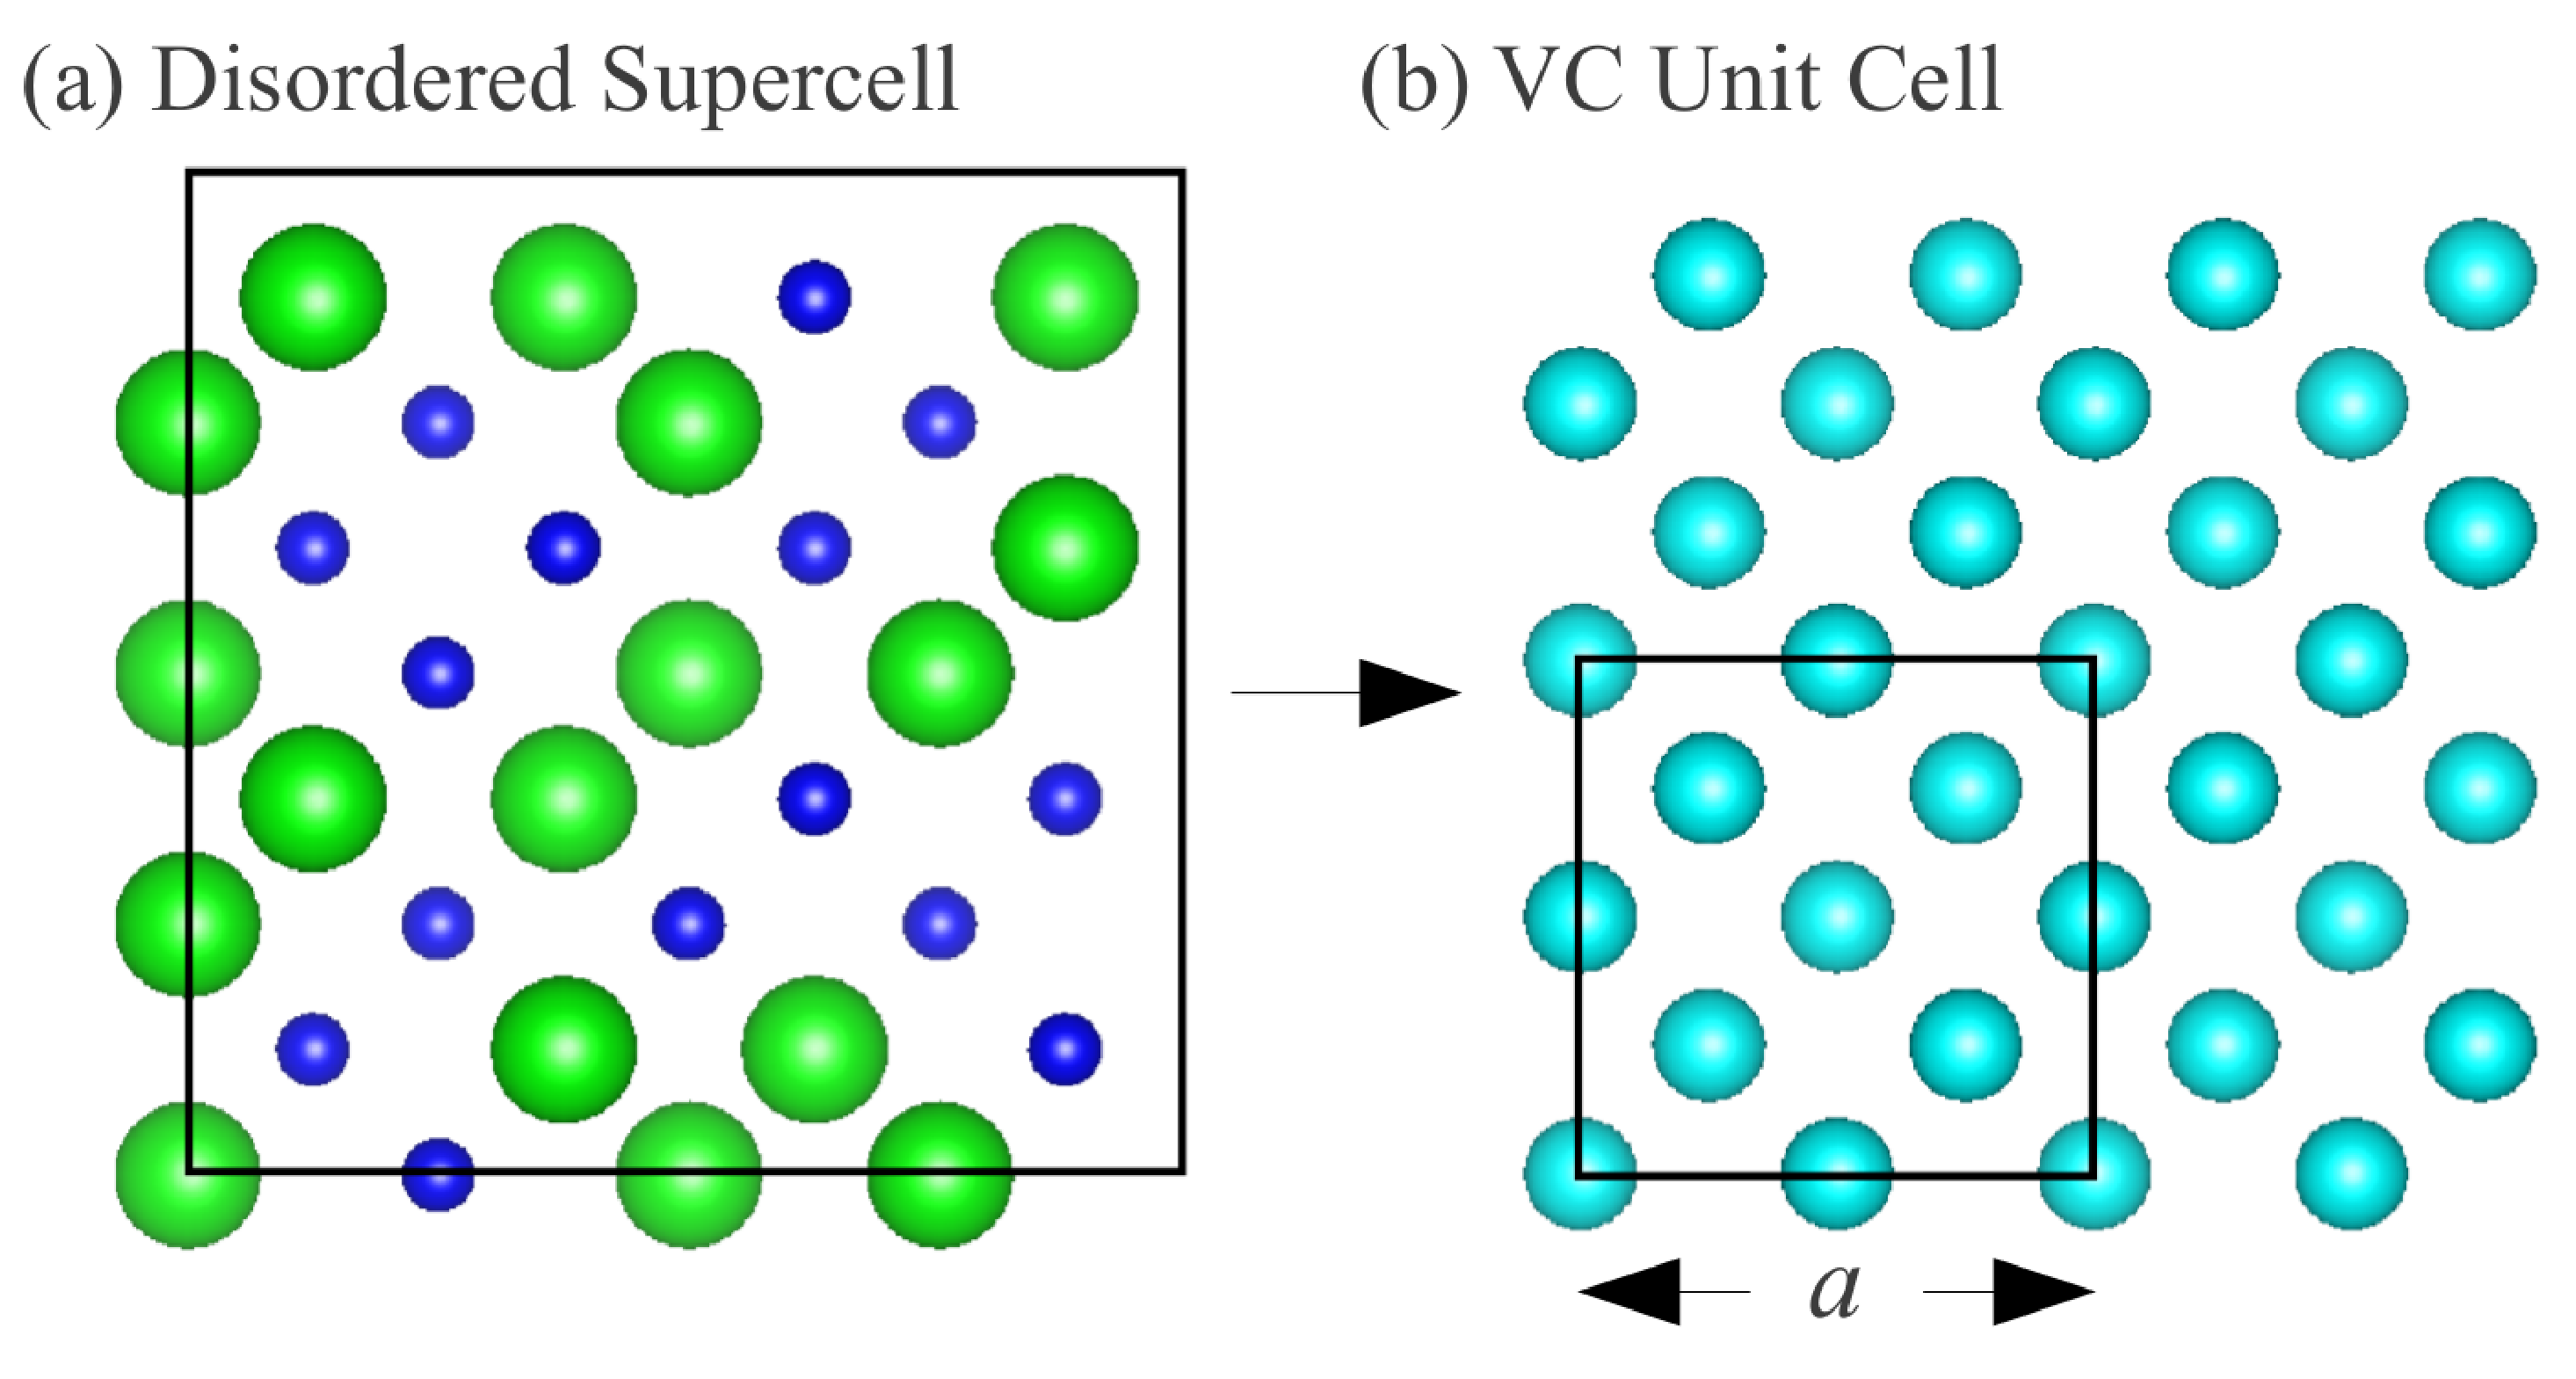
\includegraphics[scale=0.2]
{/home/jason/disorder/paper/vc/m_supercell_gimp_2.eps}
\end{center}
\caption{\label{F:supercells} 
(a) Explicitly disordered alloy supercell of 
silicon and ``heavy'' silicon ([100] direction into the page).
\cite{momma_vesta:_2008} 
(b) Equivalent VC supercell with one averaged mass. 
The sphere size represents increasing mass only, no bond disorder 
is considered. The 8-atom conventional cubic unit cell is shown 
in (b). 
}
\end{figure}
%--------------------------------------------------------------------------

\clearpage

%--------------------------------------------------------------------------
\subsection{\label{S:Calculation}Calculation and Simulation Details}
%--------------------------------------------------------------------------

The key to explicitly incorporating the effects of disorder 
is to use large disordered supercells. 
Perfect and disordered lattice supercells are generated using the 
conventional unit cells for LJ argon ($n=4$) and 
SW silicon ($n=8$), where $n$ is the number of atoms 
in the unit cell. 
Supercells are built cubically with size $N_0$, where $N_0$ is the 
number of unit cell repetitions in the three  
spatial directions. Supercells up to $N_0 = 12$ 
(6,096 atoms) are used for the LJ argon calculations. For SW silicon, 
$N_0 = 8$ (4,096 atoms) is used for 
the MD-based NMD calculations and $N_0 \le 42$ (592,704 atoms) 
is used for the MD-based GK and VC-ALD.  

Disorder is created by randomly specifying the masses of the atoms 
on the lattice. 
The composition of each lattice is labeled by $m^i_{1-c}m^j_{c}$,  
where (i) $m^i=1$ and $m^j=3$ in 
LJ units for argon, and (ii) $m^i=m_{Si}$ and $m^j=2.6m_{Si}$ 
for SW silicon and ``heavy silicon'', which has the mass of germanium. 
Concentrations, $c$, of $0,0.05,0.15$ and $0.5$ are considered. 
% Based on the previous works of others, we only consider mass disorder.

For LJ argon, the lattice constant 
at a temperature of 10 K is $5.290 \AA$.\cite{mcgaughey_phonon_2004} 
The MD simulations were performed using LAMMPS.\cite{plimpton_fast_1995} 
Efficient MD 
codes like LAMMPS scale linearly with the number of atoms in 
the system, $N_a$, which makes the GK method (see Section 
\ref{S:Thermal Conductivity}) 
computationally-inexpensive when used with empirical potentials. 
An amorphous LJ phase, discussed in Section \ref{S:Diffusivities}, 
was created by liquefying the crystal 
and instantly quenching by removing all kinetic energy.  The energy 
of the resulting structure was minimized and then annealed in an 
$NPT$ (constant number of atoms $N$, pressure $P$, and temperature $T$) 
ensemble at zero pressure and a temperature of 10 K.  
The effective zero-pressure lattice constant  
of the amorphous phase at this temperature, based on the atomic 
density, is $5.389 \AA$.  
For SW silicon, we use a lattice constant of 5.43 $\AA$ 
for all calculations, which brings the perfect crystal GK 
thermal conductivity predictions at a temperature of 300 K
\cite{goicochea_thermal_2010,he_lattice_2012} 
into better agreement with ALD predictions\cite{sellan_cross-plane_2010} 
compared to using the zero-pressure lattice constant. 

All MD simulations are first equilibrated in a $NVT$ (constant 
number of atoms, volume, and temperature) ensemble for 
$10^6$ time steps. Data is then collected from simulations in the $NVE$ 
(constant number of 
atoms, volume, and total energy) ensemble. For LJ argon, the potential 
energy is cutoff and shifted at $8.5 \AA$ (the force is not adjusted). 
Time steps of 4.285 and 0.5 fs were used for the LJ argon and 
SW silicon simulations. The same atomic trajectories are used for the 
NMD and GK methods. 

%--------------------------------------------------------------------------
\section{\label{S:Vibrational}
Vibrational Mode Properties in Alloys}
%--------------------------------------------------------------------------

%--------------------------------------------------------------------------
\subsection{\label{S:VC Gamma DOS}Density of States}
%--------------------------------------------------------------------------

In this section, we begin to examine the effects of explicitly including 
disorder by computing the frequencies and density of states (DOS)  
for the vibrational modes of disordered LJ lattice supercells and their 
equivalent VCs. The frequencies 
are computed using harmonic lattice dynamics calculations with  
GULP.\cite{gale_general_2003}  For the 
VC, the allowed wave vectors are set by $N_0$ and, due to the use of the 
conventional unit cell, there are 12 
polarization branches per wave vector.  
For the disordered supercells (referred to herein as Gamma),
the only allowed wave vector is the gamma-point (i.e., $\pmb{\kappa}=0$),  
where there are 12$N_0^3$ polarization branches. Calculation of the 
Gamma modes require the eigenvalue solution of a dynamical matrix of size 
$(3N_a)^2$ that scales as $[(3N_a)^2]^3$, limiting the system 
sizes that can be considered. This eigenvalue solution is also 
required to perform the Gamma-NMD (see Section \ref{S:From VC Gamma})  
and AF calculations (see Section \ref{S:Diffusivities}). 

The DOS for the VC and Gamma modes are plotted in Figs. \ref{F:DOS}(a), 
\ref{F:DOS}(b), and \ref{F:DOS}(c) 
for concentrations of 0.05, 0.15 and 0.5 for 
$N_0=12$ (6,912 atoms). The VC and Gamma DOS 
agree at low frequencies for all concentrations, 
where they follow the prediction of the Debye approximation that 
the DOS will scale as $\omega^2$.\cite{ashcroft_solid_1976} 
Similar agreement between VC and Gamma DOS at low frequencies 
was found in DFT predictions 
for Si$_c$Ge$_{1-c}$\cite{garg_role_2011} and 
classical models of amorphous Si$_c$Ge$_{1-c}$.
\cite{bouchard_vibrational_1988} The Debye approximation 
underpredicts the DOS at moderate frequency, which is due to 
non-linearities in the dispersion,\cite{ashcroft_solid_1976} but the 
VC and Gamma predictions remain in good agreement. 

The increasing average atomic  
mass with increasing concentration for the VC shifts all   
frequencies downward by a factor $1/[(1-c)m^i + cm^j]^{1/2}$. 
The increasing average atomic 
mass for the Gamma modes also reduces the frequencies, but not in a 
systematic manner. 
The effect of the disorder is seen at frequencies greater than 
ten by a broadening and shift of the Gamma DOS to higher frequencies 
because of the explicit use of light atoms in the supercell. This effect 
becomes more pronounced as the concentration increases.  
Duda et al. 
observed similar high-frequency broadening effects in model LJ alloys.
\cite{duda_reducing_2011} The high-frequency broadening is an indication 
of phonon localization, which is known to first occur at the 
Brillouin zone edge.\cite{chu_effect_1989} 
Based on the DOS, the vibrational modes of the explicitly disordered 
supercells at low frequencies are phonon-like, while the broadening 
of the DOS at high-frequency indicates that the Gamma 
vibrational modes may differ from the VC phonon modes in this regime. 
This behavior is further investigated in the next three sections. 

%--------------------------------------------------------------------------
\begin{figure}
\begin{center}
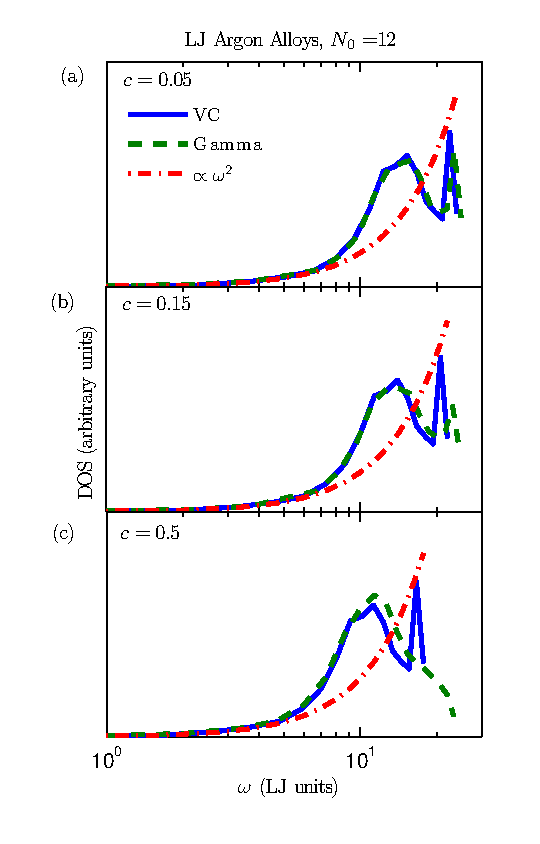
\includegraphics[scale=1.0]
{/home/jason/disorder/paper/vc/lj_alloy_dos_c05-5_5.eps}
\vspace*{-5mm}
\end{center}
\caption{\label{F:DOS} Vibrational DOS for LJ alloys calculated using the 
VC approximation and an explicitly disordered supercell 
(labeled Gamma) for concentrations (a) 0.05, (b) 0.15, and (c) 0.5. 
VC and Gamma show similar low-frequency behavior for all concentrations. 
For increasing concentrations, the frequencies of both VC 
and Gamma decrease, while the high frequency DOS for Gamma spreads and  
reaches to a higher maximum frequency because of the explicit disorder. 
The supercells are of size $N_0 = 12$ (6,912 atoms).
}
\end{figure}
%--------------------------------------------------------------------------

\clearpage

%--------------------------------------------------------------------------
\subsection{\label{S:Dispersion}Dispersion and Group Velocity}
%--------------------------------------------------------------------------

The group velocity vector in a VC is defined as the gradient of the 
dispersion curve, 
\begin{equation}\label{EQ:Dynamical}
\pmb{\text{v}}_{g,\mathbf{n}}\kv = \frac{\partial \omega\kv}{\partial \pmb{\kappa}}.
\end{equation}
We calculate the group velocities for the VC  
using finite differences on the frequencies calculated from 
harmonic lattice dynamics.\cite{mcgaughey_phonon_2006}

For a disordered solid, the three acoustic group 
velocities (two transverse and one 
longitudinal) can be predicted using the elastic constants
\cite{gale_general_2003} 
or by finite differencing of the three lowest frequency branches 
of the dispersion relation of the supercell.
\cite{he_thermal_2011,he_heat_2011} 
Except for this low-frequency behavior, there is not an 
accepted method to predict the group velocity of a 
vibrational mode in a disordered system, although there have been 
attempts.
\cite{cahill_lattice_1988,duda_reducing_2011,donadio_atomistic_2009,
he_heat_2011,he_thermal_2011} 
In the Cahill-Pohl (CP) model, for example, the group velocity of 
all disordered modes is the sound speed, $v_s$, which is also assumed  
for the HS model, Eq. \eqref{EQ:M:k_AF,HS}.
\cite{cahill_lattice_1988} This assumption is not generally valid  
for any material.\cite{feldman_numerical_1999,duda_reducing_2011,
donadio_atomistic_2009,he_heat_2011,he_thermal_2011}

Calculating the structure factors of the supercell Gamma   
modes is a method to test for their plane-wave 
character at a particular wave vector and 
polarization corresponding to the VC. 
\cite{allen_diffusons_1999,feldman_numerical_1999} 
Feldman et al. used the structure factor to predict an effective 
dispersion for a model of amorphous silicon, but did not predict 
group velocities.\cite{feldman_numerical_1999} 
Volz and Chen used the dynamic structure factor to predict the
dispersion of crystalline SW silicon using MD simulation.
\cite{volz_molecular-dynamics_2000}

The structure factor at a VC wave vector 
$\pmb{\kappa}_{VC}$ is defined as\cite{allen_diffusons_1999} 
\begin{equation}\label{EQ:SLT}
S^{L,T}\kvcw = 
\sum_{\nu} E^{L,T}\kvcv
\delta [\omega-\omega\kgv],
\end{equation}
where the summation is over the Gamma modes, $E^{T}$ refers 
to the transverse polarization and is defined as
\begin{equation}\label{EQ:EL}
E^L\kvcv = 
\left|
\sum_{b} 
\hat{\pmb{\kappa}}_{VC} \cdot e\kgvba 
\EXP{i\pmb{\kappa}_{VC}\cdot\pmb{r}_0\ab{l=0}{b}} 
\right|^2
\end{equation}
and $E^{L}$ refers to the longitudinal polarization and is defined as
\begin{equation}\label{EQ:ET}
E^T\kvcv = 
\left|
\sum_{b} 
\hat{\pmb{\kappa}}_{VC} \times e\kgvba 
\EXP{i\pmb{\kappa}_{VC}\cdot\pmb{r}_0\ab{l=0}{b}} 
\right|^2.
\end{equation}
In Eqs. \eqref{EQ:EL} and \eqref{EQ:ET}, the $b$ summations are 
over the atoms in the disordered supercell, 
$\pmb{r}_0\ab{l=0}{b}$ refers to the equilibrium atomic position of 
atom $b$ in the supercell, $l$ labels the unit cells 
($l=0$ for the supercell), 
$\alpha$ labels the Cartesian coordinates, and 
$\hat{\pmb{\kappa}}_{VC}$ is a unit vector.  
Explicit disorder is included in the Gamma frequencies 
$\omega\kgv$ and the $3N_a$ components of the eigenvectors, $e\kgvba$.

Physically, $S^{L,T}\kw$ represents  
the frequency spectrum required to create a wavepacket with a 
well-defined wave vector and polarization.
\cite{allen_diffusons_1999,feldman_numerical_1999,green_density_2011} 
For a perfect lattice, the 
structure factor peaks are delta functions centered at the mode 
frequencies, indicating that the modes are pure plane-waves 
(i.e., phonons). 
A sampling of the structure factors for the LJ argon alloys 
are plotted in Fig. \ref{F:SF} for wave vectors along the [100] and [111] 
directions in the $N_0=10$ systems.\cite{vc_fn1}  
Well-defined peaks 
at all wave vectors are due to the 
lattice structure of the disordered systems. 
Typically, the structure factor for amorphous materials has well-defined 
peaks only for small wave vector.
\cite{allen_diffusons_1999,feldman_numerical_1999} 
With increasing disorder, the structure factor spreads in width,  
particularly at high frequencies, which is an indication that the 
modes are not pure plane waves. 

From Fig. \ref{F:SF}, 
an effective dispersion curve (middle panels) can be extracted by 
locating the peaks in the 
structure factors at neighboring VC wave vectors. 
The peaks in the structure factor are larger 
than the VC predicted frequencies (plotted as solid lines in 
Fig. \ref{F:SF}) 
by at most $5\%$. Similar agreement is found with the disordered 
SW silicon lattice supercells.

Even though there is good agreement between the VC-predicted 
dispersion curves and the peaks in the structure factors from 
Fig. \ref{F:SF}, the effect of the width of the peaks is not clear. 
We will use the group velocities predicted by the VC dispersion for 
both LJ argon and SW silicon in the VC-NMD and VC-ALD calculations 
for consistency and simplicity. The validity of this 
group velocity choice will be discussed in Section \ref{S:Discussion}. 


%--------------------------------------------------------------------------
\begin{figure}
\begin{center}
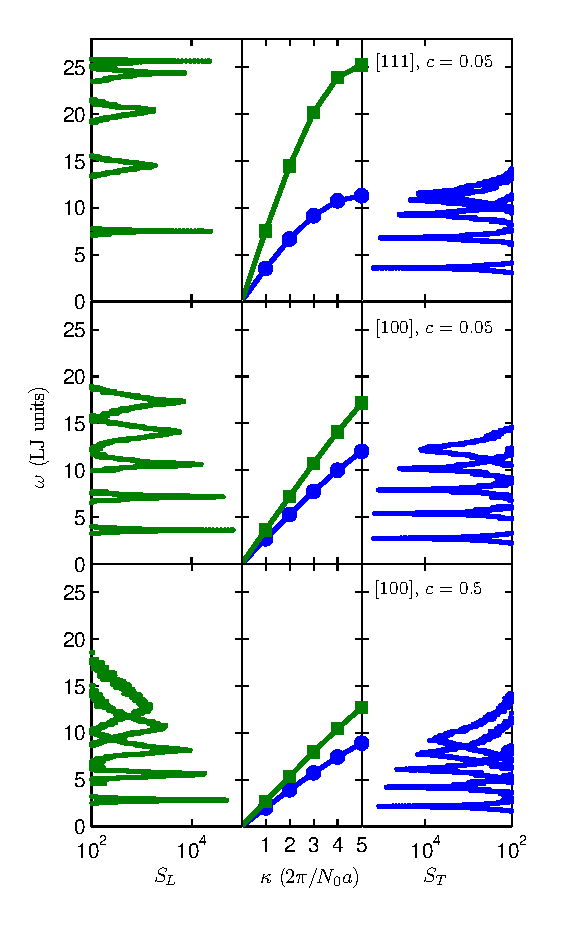
\includegraphics[scale=1.0]
{/home/jason/disorder/paper/vc/lj_alloy_dsf_100_111-3.eps}
\vspace*{-5mm}
\end{center}
\caption{\label{F:SF} 
Left and right panels: 
The structure factor for longitudinal ($S_L$) and transverse ($S_T$) 
polarizations along high-symmetry directions  
of the mass disordered LJ argon supercells ($N_0=10$, $c=0.05,0.5$).  
Center panels:
The VC predicted dispersion curves (solid lines) agree well with the 
locations of the peaks in $S_{L}$ and $S_{T}$. The wavenumber axis 
in the center panel is normalized by the maximum value of the wavenumber  
in the given direction. 
}
\end{figure}
%--------------------------------------------------------------------------

\clearpage

%--------------------------------------------------------------------------
\subsection{\label{S:Phonon Lifetimes}Lifetimes}
%--------------------------------------------------------------------------

%--------------------------------------------------------------------------
\subsubsection{\label{S:From VC Gamma}From VC-NMD and Gamma-NMD}
%--------------------------------------------------------------------------

Once the group velocities are predicted using the VC dispersion, 
the mode lifetimes are required to predict the thermal 
conductivity using Eq. \eqref{EQ:k_vib}. 
As an alternative to the VC-ALD approach for predicting lifetimes, 
which is discussed in the next section,  
we first use the MD simulation-based 
NMD method.\cite{ladd_lattice_1986,mcgaughey_quantitative_2004,
turney_predicting_2009-1,larkin_comparison_2012} In NMD, the 
atomic trajectories are first mapped onto the vibrational 
mode coordinate $q\kvt$ and its time derivative $\dot{q}\kvt$ by
\cite{dove_introduction_1993}
\begin{equation}\label{EQ:q}
\begin{split}
q\kvt=&\SUM{0}{}\sqrt{\frac{m_b}{N}}u_{\alpha}\lbt e^*\kvba
\EXP{i\pmb{\kappa}\cdot\mathbf{r}_0\ab{l}{0}}
\end{split}
\end{equation}
and
\begin{equation}\label{EQ:qdot}
\begin{split}
\dot{q}\kvt{}{}{}=&\SUM{0}{}\sqrt{\frac{m_b}{N}}\dot{u}_{\alpha}
\lbt e^*\kvba\EXP{i\pmb{\kappa}\cdot\mathbf{r}_0\ab{l}{0}}.
\end{split}
\end{equation}
Here, $m_b$ is the mass of the $b_{th}$ atom in the unit cell, 
$u_{\alpha}$ is the $\alpha$-component of the atomic displacement 
from equilibrium, $\dot{u}_{\alpha}$ is the $\alpha$-component 
of the atomic velocity, and $t$ is time.    
The total energy of each vibrational mode, $E\kvt$, is calculated 
from 
\begin{equation}\label{A:E}
\begin{split}
E\kvt = \frac{\omega\kv^2}{2} q\kvt^*q\kvt + 
\frac{1}{2}\dot{q}\kvt^*\dot{q}\kvt.
\end{split}
\end{equation}
The vibrational mode lifetime is predicted using 
\begin{equation}\label{EQ:tau_nmd}
\tau\kv = \int_{0}^{t^*}
\frac{<E\kvt E\kvzero>}{ <E\kvzero E\kvzero> }dt,
\end{equation}
where the upper integration limit $t^*$ is set to be much larger 
than the mode lifetime and the brackets indicate 
an ensemble average.\cite{larkin_comparison_2012} 
Equation \eqref{EQ:tau_nmd} 
is derived by assuming that the energy autocorrelation follows an 
exponential decay.\cite{ladd_lattice_1986,turney_predicting_2009-1} 
The NMD calculations scale 
as $(N_a)^2$.\cite{turney_predicting_2009}  

We perform the MD simulations using the fully disordered supercells  
and project onto the frequencies and eigenvectors 
from both the VC unit cell [$\omega\kv$, $e\kvba$] and the 
Gamma supercell [$\omega\kgv$, $e\kgvba$]. 
The trajectories from 
these MD simulations are also used in the GK method calculations
(Section \ref{S:Thermal Conductivity}). 
The MD simulations were ten times longer than the 
longest lifetime in the system, which was  
estimated from the VC-ALD predicted lifetimes. For LJ 
argon and SW silicon, data was collected for $2^{20}$ and 
$2^{22}$ time steps and the atomic trajectories were sampled 
every $2^8$ and $2^4$ time steps. 
Ensemble averaging of the energy autocorrelations was performed 
using ten independent, initially-randomized velocity distributions. 

For the normal modes of the lattice supercell, 
Eq.~\eqref{EQ:tau_nmd} is exact, but this expression becomes an 
approximation when 
using the VC normal modes to perform the mappings in Eqs.  
\eqref{EQ:q} and \eqref{EQ:qdot}. 
Even for larger disorder ($c=0.5$),  
where the energy autocorrelations 
deviate from an exponential decay, 
an effective lifetime can still be predicted 
using Eq. \eqref{EQ:tau_nmd} (see Appendix \ref{A:NMD XCORR}). 
The lifetimes predicted using VC-NMD and Gamma-NMD  
are shown in Figs. \ref{F:VC Gamma life}(a)-\ref{F:VC Gamma life}(d) 
for the LJ argon crystal and all alloys at a temperature of 10 K. 
The range of frequencies for 
VC-NMD and Gamma-NMD differ slightly due to differences in 
the DOS (see Fig. \ref{F:DOS}). 
For a small interval of frequency, there is a wider range of 
predicted lifetimes for Gamma-NMD. This spread is because there 
is no symmetry-averaging of the mode properties, 
which is possible for the VC by considering the crystal 
lattice's irreducible BZ.\cite{ashcroft_solid_1976} 

The lifetimes predicted by both VC-NMD and Gamma-NMD 
show a $\omega^{-2}$ scaling at low frequency and a $\omega^{-4}$ 
scaling (for the alloys) and 
even faster for mid-range frequencies. The $\omega^{-2}$ scaling 
is due to three-phonon scattering processes
\cite{callaway_model_1959,maradudin_scattering_1962}. The 
$\omega^{-4}$ scaling is due to phonon-mass point defect 
scattering.\cite{klemens_scattering_1955,klemens_thermal_1957,
mattis_phonon_1957,tamura_isotope_1983} 
A constant lifetime is observed at the highest frequencies  
for both VC-NMD and Gamma-NMD except at $c=0.5$ for VC-NMD. We are not 
aware of any theoretical prediction of this high-frequency behavior.

The majority of the lifetimes predicted by both VC-NMD and 
Gamma-NMD are larger than the Ioffe-Regel (IR) limit,
\cite{taraskin_determination_1999} 
\begin{equation}\label{EQ:IR}
\tau = \frac{2\pi}{\omega}.
\end{equation}
The physical interpretation of the IR limit is a mode that  
scatters in a time equal to its oscillation period. Our results suggest 
that the IR limit is a good lower-limit for the lifetimes predicted 
by VC-NMD and Gamma-NMD 
for LJ argon (Fig. \ref{F:VC Gamma life}) 
and VC-NMD for SW silicon [see Fig. \ref{F:Dph_si}(a) in 
Section \ref{S:SW}]. 

Overall, good agreement is seen in the predicted lifetimes from VC-NMD and 
Gamma-NMD in both magnitude and trends. The use of the VC normal modes 
is an approximation that becomes worse as the concentration is increased 
(see Appendix \ref{A:NMD XCORR}), but our results suggest that the effect 
is only pronounced at the highest frequencies and at high alloy 
concentrations. 
The only approximation associated with Gamma-NMD is the use  
of the harmonic lattice dynamics-predicted frequencies and eigenvectors 
to map the atomic trajectories from the fully anharmonic MD simulations. 
This assumption has been shown to be valid for LJ argon below temperatures 
of 40 K.\cite{turney_predicting_2009-1} 
Based on the good agreement with Gamma-NMD, the 
VC-NMD lifetimes are used along with the VC group velocities to 
predict thermal conductivity in Section \ref{S:Thermal Conductivity}. 
For Gamma-NMD, there is no accepted way to predict the mode 
group velocities, so that the thermal conductivity cannot be predicted 
using Eq. \eqref{EQ:k_vib}. 

%--------------------------------------------------------------------------
\begin{figure}
\begin{center}
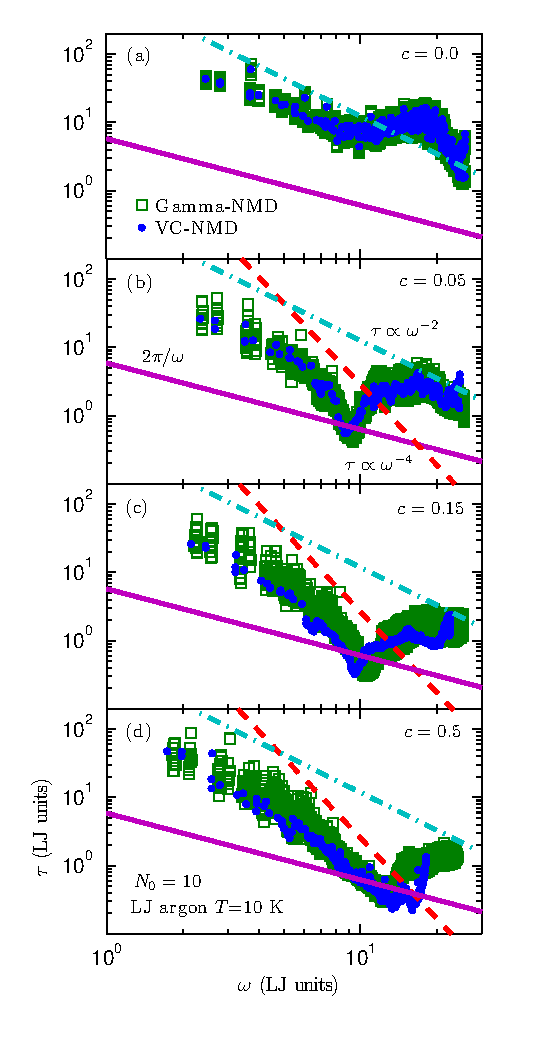
\includegraphics[scale=1.0]
{/home/jason/disorder/paper/vc/lj_alloy_nmd_vc_gamma_life-3.eps}
\vspace*{-5mm}
\end{center}
\caption{\label{F:VC Gamma life} Lifetimes predicted using VC-NMD 
and Gamma-NMD from MD simulations of (a) perfect LJ argon and 
(b),(c),(d) mass-disordered LJ alloys for $N_0=10$. 
$\omega^{-2}$ and $\omega^{-4}$ 
scalings are observed at low to mid frequencies. 
For both VC-NMD and Gamma-NMD, most mode 
lifetimes are greater than the Ioffe-Regel limit $\tau = 2\pi/\omega$. 
\cite{taraskin_determination_1999}
While there is more scatter in the Gamma-NMD data 
(see Section \ref{S:From VC Gamma}), the lifetime magnitudes and 
trends agree well, an important consideration when comparing the 
VC-NMD and VC-ALD lifetimes in Fig. \ref{F:Dph_lj}(a).
}
\end{figure}
%--------------------------------------------------------------------------

\clearpage

%--------------------------------------------------------------------------
\subsubsection{\label{S:From VC-ALD}From VC-ALD}
%--------------------------------------------------------------------------

Under the VC approximation, the 
ALD calculations\cite{turney_predicting_2009-1} are performed on the 
conventional unit cells of LJ argon and SW silicon with a single  
atomic mass based on the alloy concentration. The ALD calculations scale 
as $b^4$ and $(N_{0})^2$.\cite{turney_predicting_2009} Disorder is not included 
explicitly but is treated using perturbation theory. 
Assuming phonon scattering mechanisms 
to operate independently, the 
effective phonon lifetime can be found using the Matthiessen rule,
\cite{ziman_electrons_2001} 
\begin{equation}\label{EQ:Matthiessen}
\frac{1}{\tau\kv} = \frac{1}{\tau_{p-p}\kv} + \frac{1}{\tau_{p-d}\kv},
\end{equation}
where $\tau_{p-p}\kv$ accounts for intrinsic phonon-phonon scattering 
and $\tau_{p-d}\kv$ accounts for phonon-defect scattering.

Phonon-phonon scattering in ALD is modeled by including three-phonon 
processes.\cite{turney_predicting_2009-1,garg_role_2011,tian_phonon_2012} 
The present study is concerned with temperatures much less than the 
melting temperature of either LJ argon
\cite{mcgaughey_phonon_2004} or 
SW silicon\cite{stillinger_computer_1985} so that we believe the effects 
of higher-order phonon processes are 
negligible.\cite{ecsedy_thermal_1977,turney_predicting_2009-1} 
We predict the phonon-phonon lifetimes using the method 
described in Ref. \citenum{turney_predicting_2009-1}, 
with all classical expressions for the populations to remain 
consistent with the classical MD-based methods from 
Section \ref{S:From VC Gamma}. 

Using perturbation theory, Tamura derived a general expression for 
phonon scattering by mass point defects to second order that was applied 
to study isotopic germanium.\cite{tamura_isotope_1983}   
By considering the symmetry properties of the FCC lattices 
considered in this work, his expression reduces to 
\begin{equation}\label{EQ:taud_dos}
\begin{split}
\frac{1}{\tau_{p-d}\kv} =\frac{\pi}{2} g_2 \omega^2\kv DOS[\omega\kv], 
\end{split}
\end{equation}
where  
\begin{equation}\label{EQ:gn}
\begin{split}
g_n = \sum_\mu c^{\mu}(1-m^{\mu}/\bar{m}^{\mu})^n.
\end{split}
\end{equation}
Here, $c^\mu$ and $m^\mu$ are the concentration and  
mass of the $\mu$-th species 
and $\bar{m}^{\mu}$ is the average mass. Bond disorder 
can be accounted for using a similar expression with an average
atomic radius or suitable scattering cross-section.
\cite{klemens_scattering_1955,klemens_thermal_1957} 
For the binary LJ argon and SW silicon alloys considered here, 
there is one atom type in the unit cell  
with $\mu=i,j$, so that the alloying atom labeled by $m^j_{c}$ 
can be considered to be an ``isotope'' of the atom labeled 
$m^i_{1-c}$.

The lifetimes predicted by VC-ALD for LJ argon at a concentration 
of 0.05 are plotted in Fig. \ref{F:Dph_lj}(a).\cite{vc_fn2}    
Also plotted are the lifetimes for the perfect system and from the 
VC-NMD predictions [Fig. \ref{F:VC Gamma life}(b)] at this 
concentration. At low frequencies, where the DOS is Debye-like 
[$D(\omega) \propto \omega^{2}$, Fig. \ref{F:DOS}], 
$\tau_{p-p}\kv$ scales as $\omega^{-2}$, 
a scaling also observed in the VC-NMD and Gamma-NMD lifetimes. 
Under the Debye-approximation, 
the phonon scattering due to mass point-defects 
is predicted to scale as $\omega^{-4}$ from Eq. \eqref{EQ:taud_dos}.
\cite{mattis_phonon_1957,tamura_isotope_1983} 
This scaling is observed in the VC-NMD, Gamma-NMD, and VC-ALD 
predicted lifetimes in the mid-frequency range.  
VC-ALD does not predict the frequency-independent lifetimes 
at high frequency for LJ argon observed in VC-NMD and Gamma-NMD,  
and a significant number fall below the IR limit. 
The lifetimes predicted by 
NMD and ALD for the perfect LJ argon crystal agree 
within 20$\%$ on a mode-by-mode basis, and the 
resulting thermal conductivities agree within their uncertainties 
(see Table \ref{T:cond_table}).
% The disorder 
% scattering scaling is expected to fall off faster than $\omega^{-4}$ 
% when $D(\omega)$ grows faster than the Debye scaling of 
% $\omega^{2}$ (Fig. , Section ). 
% The lifetimes do fall off faster $\omega^{-4}$ for the 
% mass disordered LJ FCC supercells for a narrow range of 
% frequencies near $\omega = 10$ in Fig. for $c=0.05,0.15$, 
% but seem to follow more closely $\omega^{-4}$ for $c=0.5$. 

The Tamura theory was developed to predict the reduction of lifetimes 
in isotopic germanium, which is only weakly disordered 
($\sim$ 5$\%$ variation in the atomic masses). In the LJ alloys, the 
masses differ by a factor of three. Large mass ratios were also 
considered in DFT VC-ALD studies of SiGe  
(mass ratio of 2.6)\cite{garg_role_2011}, 
PbTeSe (2.6)\cite{tian_phonon_2012}, 
and MgSiSn (4.9)\cite{li_thermal_2012}. 
The importance of higher-order interactions in 
the Tamura theory can be estimated by the disorder strength 
(i.e., $g_n$ for $n > 2$).\cite{tamura_isotope_1983} 
For isotopically-disordered germanium, Tamura estimated that the 
higher-order contributions were negligible ($g_2 = 5.87\times10^{-4}$, 
$g_3 \sim 10^{-7}$ and $g_4 \sim 10^{-7}$).\cite{tamura_isotope_1983} 
For LJ argon at a concentration of 0.15,  
$g_2 = 0.3018$, $g_3 = -0.3250$ and $g_4 = 0.4411$. 
It is possible that the neglect of the higher-order interactions 
in the Tamura theory is responsible for the 
discrepancy of the lifetimes predicted by VC-NMD and Gamma-NMD 
versus VC-ALD at high frequencies. Full evaluation of the 
higher-order interactions in the Tamura theory is of similar 
complexity to anharmonic phonon interaction,
\cite{maradudin_scattering_1962,ecsedy_thermal_1977,
turney_predicting_2009-1} and is beyond the scope of this work.

%--------------------------------------------------------------------------
\begin{figure}
\begin{center}
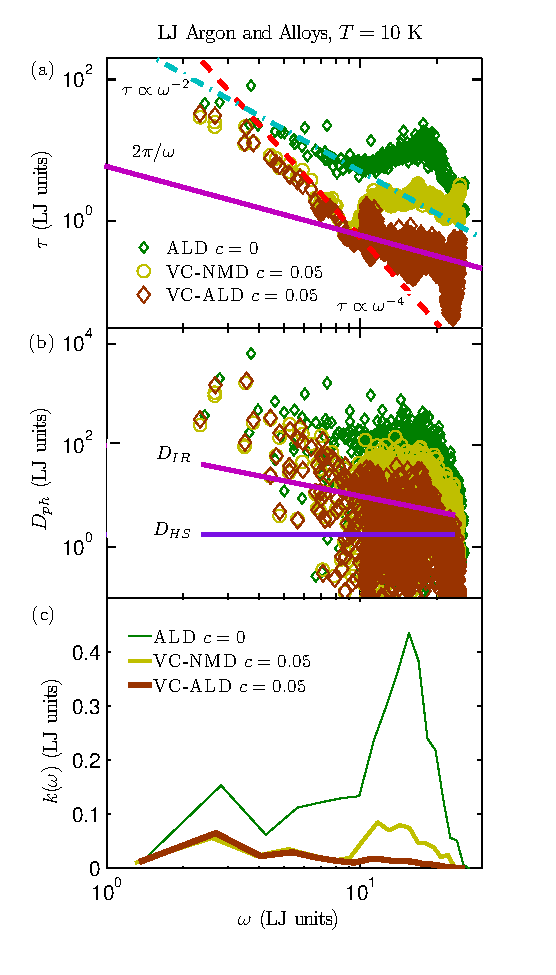
\includegraphics[scale=1.0]
{/home/jason/disorder/paper/vc/af_nmd_ald_tau_diff_kw_c05_3-4.eps}
\vspace*{-5mm}
\end{center}
\caption{\label{F:Dph_lj} (a) Predicted lifetimes using 
VC-NMD and VC-ALD for LJ argon ($T=10$ K, $N_0=10$, and $c=0.05$).  
(b) Mode diffusivities compared  
to the HS limit, $D_{HS}$ [Eq. \eqref{EQ:M:D_HS}], and IR limit, 
$D_{IR}$ [Eq. \eqref{EQ:M:D_IR}]. 
VC-NMD and VC-ALD predict 
a large number of high-frequency modes with $D_{ph} < D_{HS}$. 
(c) Thermal conductivity frequency spectrum, 
which peaks at high frequency, in contrast to SW silicon 
[(Fig. \ref{F:Dph_si}(c)].}
\end{figure}
%--------------------------------------------------------------------------

\clearpage

% NOT USED:
% $c=0.001$ $g_3 = -0.0079$, $g_4 = 0.0158$,
% $c=0.001$ $g_3 = -0.0079$, $g_4 = 0.0158$,
% $c=0.01$ $g_3 = -0.073$, $g_4 = 0.142$,   
% $c=0.15$ $g_3 = -0.325$, $g_4 = 0.441$
% $c=0.5$ $g_3 = 0.0$, $g_4 = 0.0625$

%--------------------------------------------------------------------------
\subsection{\label{S:Diffusivities}
Diffusivities}
%--------------------------------------------------------------------------

We now use the AF theory to provide a lower limit for the contribution  
of a given vibrational mode to thermal conductivity. 
While studies have been performed on alloying the amorphous phase,
\cite{feldman_thermal_1993} the 
AF theory has not been previously applied to disordered lattices. In the 
classical, harmonic limit for specific heat, a mode's contribution to the 
thermal conductivity of is determined by its diffusivity, 
\begin{equation}\label{EQ:Dph}
D_{ph,\mathbf{n}}\kv = v^2_{g,\mathbf{n}}\kv \tau\kv, 
\end{equation}
such that from Eq. \eqref{EQ:k_vib} 
\begin{equation}\label{EQ:k_Dph}
k_{ph,\mathbf{n}} = \sum_{\pmb{\kappa}} \sum_{\nu} 
\frac{k_{\text{B}}}{V} D_{ph,\mathbf{n}}\kv.
\end{equation} The lower limit for phonon diffusivity is 
zero since the group velocities can be zero (e.g., optical modes at the 
Brillouin zone center). 
% Even for large disorder in the alloys, modes 
% at low frequency have well-defined group velocities and lifetimes, which 
% is demonstrated by the supercell structure factor peaks 
% (see Fig. \ref{F:SF}) and 
% lifetimes predicted by VC-NMD, Gamma-NMD, and VC-ALD 
% [see Figs. \ref{F:VC Gamma life}, \ref{F:Dph_lj}(a)].  

In the HS limit,\cite{cahill_lattice_1988} 
the diffusivity of each mode is
\begin{equation}\label{EQ:M:D_HS}
D_{HS} = \frac{1}{3} v_s a,
\end{equation}
which leads to Eq. \eqref{EQ:M:k_AF,HS}. 
The physical interpretation of Eq.~\eqref{EQ:M:D_HS} 
is that all vibrational modes transport heat at the sound speed 
and have a mean free path of the lattice spacing. 
Based on the IR limit, another possible lower-bound of 
diffusivity is  
\begin{equation}\label{EQ:M:D_IR}
D_{IR} = \frac{2\pi}{3} \frac{v^2_s}{\omega}. 
\end{equation} 
To evaluate Eqs. \eqref{EQ:M:D_HS} and \eqref{EQ:M:D_IR}, 
the sound speed is estimated by 
\begin{equation}\label{EQ:M:vs}
v_s = \frac{1}{3}v_{s,L} + \frac{2}{3}v_{s,T},
\end{equation}
where $v_{s,L}$ and $v_{s,T}$ are the longitudinal and transverse 
sound speeds calculated from the elastic constants,
\cite{gale_general_2003} which agree within 20$\%$ with the 
branch-averaged sound speeds along the high-symmetry dispersion 
directions [100],[110], and [111]. For LJ argon and SW silicon, 
$v_s = 6.93$ (LJ units) and $5,790$ m/s. 
The CP model assumes Eq. \eqref{EQ:M:D_IR} for the mode 
diffusivities.\cite{cahill_lattice_1988} 
As seen in Fig.~\ref{F:Dph_lj}(b) for the LJ argon alloy at 
a concentration of 0.05, VC-NMD and VC-ALD predict [from 
Eq. \eqref{EQ:Dph}, using the $x$-component of group velocity], a 
significant number of modes with  
$D_{ph}\kv$ less than $D_{HS}$, and $D_{IR}$ approaches $D_{HS}$ at 
high frequencies. For both VC-NMD and VC-ALD, we 
approximate $\pmb{\text{v}}_{g,\mathbf{n}}\kv$ from the VC dispersion 
(Section \ref{S:Dispersion}) so that any differences in 
diffusivity $D_{ph}$ will come from the predicted lifetimes.  

In a disordered system,  
modes can transport heat by harmonic coupling in the AF theory of 
diffusons.\cite{allen_thermal_1993} 
While the HS model assumes a mode-independent diffusivity, 
the AF theory is capable of predicting mode-specific thermal 
diffusivities $D_{AF}$.
\cite{feldman_thermal_1993,feldman_numerical_1999,
shenogin_predicting_2009} Since the AF theory is harmonic, the 
diffusivities typically diverge as the frequency approaches zero 
because these vibrations are long-wavelength plane waves  
that are weakly scattered by the disorder.
\cite{sheng_introduction_2006,vitelli_heat_2010}
The mode-specific diffusivities, $D_{AF}$, of an LJ argon amorphous 
phase\cite{vc_fn4} are plotted in Fig. \ref{F:AF} along with 
$D_{HS}$ and $D_{IR}$. 
Except at the highest frequencies, the diffusivity of all amorphous 
modes can be approximated using the mode-independent diffusivity 
$D_{HS}$. The lower-limit $D_{IR}$ is clearly an overprediction 
for the amorphous mode diffusivities. Also plotted in Fig. \ref{F:AF} 
are diffusivities predicted from the AF theory for the 
explicitly-disordered LJ argon lattice supercell  
alloy at a concentration of 0.5. As expected, the AF theory 
predictions diverge at low frequency.\cite{vc_fn5} 
The diffusivity of all modes are larger than $D_{HS}$ except 
at the highest frequencies, where they tend to zero as with the amorphous 
phase. This result supports the hypothesis that the lower-bound of the 
VC predicted phonon diffusivity should be $D_{HS}$ (and not zero), 
which is further explored in Sections \ref{S:Thermal Conductivity} and 
\ref{S:SW}.

% NOT USED:
% energy transport in jammed sphere packings\cite{xu_energy_2009}
% heat transport in model jammed solids\cite{vitelli_heat_2010}

%--------------------------------------------------------------------------
\begin{figure}
\begin{center}
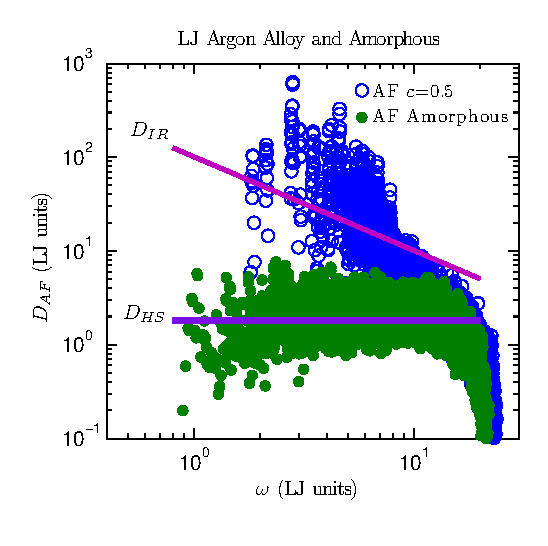
\includegraphics[scale=1.0]
{/home/jason/disorder/paper/vc/af_c5_amor_DAF_kw_3.eps}
\vspace*{-5mm}
\end{center}
\caption{\label{F:AF} AF theory predictions of disordered mode  
diffusivities for LJ argon alloy and amorphous phases. The amorphous 
phase is well-described by a 
mode-independent diffusivity $D_{HS}$ [Eq. \eqref{EQ:M:D_HS}]. The 
system size for the alloy is $N_0=10$ (6,912 atoms), and the amorphous
phase has 6,912 atoms. 
}
\end{figure}
%--------------------------------------------------------------------------

\clearpage

%--------------------------------------------------------------------------
\subsection{\label{S:Discussion}Discussion}
%--------------------------------------------------------------------------

In this section, in anticipation of the thermal conductivity predictions 
in Section \ref{S:Thermal Conductivity}, we discuss two possible sources 
of error in the VC-predicted mode properties. 
To start, we note that for disordered systems, it is generally only 
possible to assign a 
unique lifetime and group velocity to vibrational modes  
in the low-frequency, propagating limit.
\cite{feldman_numerical_1999,xu_energy_2009} The mode diffusivity 
is the fundamental transport property.
\cite{allen_thermal_1993,feldman_thermal_1993,feldman_numerical_1999} 

We believe that the VC-predicted group velocities, particularly 
for $v_{g,\mathbf{n}}\kv \approx 0$, are an underprediction of the 
velocity scale required to evaluate Eq. \eqref{EQ:Dph}.  
This statement is supported by the 
AF-theory diffusivities plotted in Fig. \ref{F:AF}, 
which are finite for the LJ alloy at a concentration 
of 0.5. While the diffusivity from Eq. \eqref{EQ:Dph} can be 
zero because of the VC predicted group velocities, this result is not 
consistent with the AF theory predictions.

The VC-NMD and Gamma-NMD predicted lifetimes are generally larger 
than the IR limit  
for LJ argon and its alloys (see Fig. \ref{F:VC Gamma life}). 
The constant lifetime observed at the highest frequencies  
for both VC-NMD (except at $c=0.5$) and Gamma-NMD is 
consistent with the plateau of mode diffusivity at high 
frequency predicted for a model disordered lattice, 
which was explained by a plateau in the vibrational mode lifetimes.
\cite{sheng_heat_1991} 
VC-ALD predicts essentially monotonically 
decreasing lifetimes with increasing frequency for the LJ argon 
alloys [Fig. \ref{F:Dph_lj}(a)] with many falling below the IR limit. 
Because VC-NMD and VC-ALD use the same values for 
$v_{g,\mathbf{n}}\kv$, the 
mode diffusivities will therefore be underpredicted for 
VC-ALD compared to VC-NMD for the LJ argon alloys because of the 
lifetime underprediction. 

% There are thus two underpredictions to consider 
% when interpreting the thermal conductivity predictions in 
% Section : (i) underprediction 
% of the diffusivity that results from using the VC group 
% velocities for 
% VC-NMD and VC-ALD, and (ii) the underprediction of the mode 
% lifetimes for LJ argon alloys by the VC-ALD perturbative models. 

% Dispersion for a model disordered 1D system demonstrated   
% the reduction of the frequency-dependent group velocities due to the 
% zone-folding effect.\cite{duda_reducing_2011} 

%--------------------------------------------------------------------------
\section{\label{S:Thermal Conductivity}Thermal Conductivity Predictions}
%--------------------------------------------------------------------------

The thermal conductivities of the LJ systems can now be predicted from 
Eq. \eqref{EQ:k_vib} using the vibrational mode properties 
from VC-NMD and VC-ALD. Given the discussion regarding the 
VC-predicted mode properties in Section \ref{S:Discussion}, 
we also predict thermal conductivity using the equilibrium 
MD-based GK method, which is a top-down method that does not make any 
approximations about the nature of the vibrational modes. 
Thermal conductivities predicted by the GK method 
naturally capture all scattering mechanisms.
\cite{landry_complex_2008,he_thermal_2011,he_lattice_2012} 
The heat current was computed every ten time steps from the same atomic 
trajectories (positions and velocities) used for the VC-NMD and 
Gamma-NMD calculations.  The thermal conductivity is 
determined from the maximum of the integral of the heat 
current autocorrelation function.

The thermal conductivities predicted by VC-NMD, VC-ALD, and GK are system 
size-dependent [i.e., $k = k(N_0)$] for all lattices and methods except 
perfect LJ argon from GK.\cite{mcgaughey_quantitative_2004} 
To predict a bulk thermal conductivity, $k_{bulk}$,  
a linear extrapolation procedure is 
used, whereby 
\begin{equation}\label{EQ:k0}
\frac{k(N_0)}{k_{bulk}} = 1 - \frac{c_0}{N_0},
\end{equation}
where $c_0$ is a constant.\cite{turney_predicting_2009,esfarjani_heat_2011,
shiomi_thermal_2011} The thermal conductivity 
is predicted for varying system sizes and the bulk thermal conductivity is 
obtained by fitting Eq. \eqref{EQ:k0} to the data. 
For VC-NMD and VC-ALD, the validity of Eq. \eqref{EQ:k0}  
requires that the low-frequency modes be dominated by 
phonon-phonon scattering (i.e., $\tau\ \propto \omega^{-2}$) and  
follow the Debye approximation 
with respect to the group velocity and DOS.
\cite{shiomi_thermal_2011,esfarjani_heat_2011} For the LJ 
argon alloys, this requirement is satisfied for modest system sizes 
(for $N_0 = 6$ to $12$) so that both VC-NMD and VC-ALD thermal 
conductivity predictions can be extrapolated to a bulk value. 

Bulk thermal conductivity predictions for the LJ argon alloys using  
VC-NMD, VC-ALD, and GK are tabulated in Table \ref{T:cond_table} 
and plotted in Fig. \ref{F:cond_lj}. Also plotted 
in Fig. \ref{F:cond_lj} is the HS  
thermal conductivity prediction $k_{HS}$ 
[Eq. \eqref{EQ:M:k_AF,HS}]. The thermal conductivity predicted 
for the LJ amorphous phase by GK is $0.17$ W/m-K,  
which is in good agreement with $k_{HS}$ (0.16 W/m-K) for the 
perfect crystal.  
The predicted thermal conductivities of the LJ argon alloys at high 
concentration are a factor of two to three larger than $k_{HS}$.  
While agreement between the three methods is found for the perfect 
crystal, VC-NMD and VC-ALD underpredict the alloy thermal 
conductivities compared to GK. 
The underprediction is modest for VC-NMD, where $k_{NMD}$ is 
$80\%$ of $k_{GK}$ or greater for all concentrations. The VC-ALD method 
significantly underpredicts the thermal conductivity of the LJ argon alloys. 
The largest deviation is at a concentration of 0.05, where 
$k_{VC-ALD}$ is $56\%$ of $k_{GK}$.

In Section \ref{S:Diffusivities}, 
we argued for the existence of a minimum mode 
diffusivity, $D_{HS}$ [Eq. \eqref{EQ:M:D_HS}]. 
As shown in Fig. \ref{F:Dph_lj}(b), the diffusivities of 
many high-frequency modes in the LJ alloys, predicted by both VC-NMD 
and VC-ALD, fall below this limit.  Based on this observation, we propose 
that any diffusivity below the limit be set to $D_{HS}$ 
for thermal conductivity prediction. 
The results of this adjustment, 
referred to as VC-NMD* and VC-ALD*, are plotted in Fig. \ref{F:cond_lj} 
and included in Table \ref{T:cond_table}.  
The adjusted thermal conductivities predicted by VC-NMD$^*$ are now  
within $10\%$ of the GK value for all concentrations, which
is within the prediction uncertainties. 
Combined with $D_{HS}$, we believe that the VC-NMD predicted 
diffusivities are good representations for the explicitly-disordered 
modes present in the MD simulations. Another possible 
adjustment, $D_{IR}$ [Eq. \eqref{EQ:M:D_IR}], results in a thermal 
conductivity of $0.94 \pm 0.09$ W/m-K for the LJ argon alloy at a 
concentration of 0.05, well above the value predicted by GK. 
We also note that the thermal 
conductivity of the amorphous phase is well-modeled by a mode-independent 
diffusivity $D_{HS}$, while $D_{IR}$ overpredicts for all modes in the 
amorphous phase (see Fig. \ref{F:AF}). 
Thus, we believe that $D_{HS}$ is the more appropriate HS limit. 

By applying the HS limit adjustment VC-ALD$^*$, the thermal 
conductivities are brought into marginally better agreement with 
the GK values, worst for a concentration of $0.05$, where 
$k_{VC-ALD^*}$ is $65\%$ of $ k_{GK}$.  
As seen in Fig. \ref{F:Dph_lj}(b), the VC-ALD method fails to 
accurately predict the high-frequency mode diffusivities for 
LJ argon alloys. Since the group velocities are the same for 
VC-NMD and VC-ALD, the underprediction of the high-frequency 
diffusivities is
due to the underprediction of the high-frequency 
mode lifetimes from VC-ALD compared to VC-NMD. We know that the 
VC-NMD predicted lifetimes are more accurate values due 
to their agreement with Gamma-NMD [Fig. \ref{F:VC Gamma life}]. 

The thermal conductivity spectrum, defined as 
the contribution to thermal conductivity of modes at a given frequency, 
is plotted in Fig. \ref{F:Dph_lj}(c) for VC-NMD and VC-ALD for the 
perfect crystal and the alloy with a concentration of 0.05. The thermal 
conductivity of LJ argon and its alloys has important 
contributions from high-frequency modes. 
VC-ALD underpredicts the high-frequency 
diffusivities compared to VC-NMD, which leads to an 
underprediction of the high-frequency thermal conductivity spectrum 
compared to VC-NMD. This result can be traced back to an underprediction 
of the high-frequency lifetimes compared to VC-NMD and Gamma-NMD 
[Fig. \ref{F:Dph_lj}(a)]. 

% The failure of the VC-ALD method can be demonstrated further 
% by moving to higher temperature $T=40$ K in Fig. \ref{F:cond_lj} a.
% The beginning breakdown of the intrinsic phonon-phonon ($\tau_{p-p}\kw$) 
% scattering model 
% can be observed for $c=0.0$ at 
% $T=40$ K (Fig. \ref{F:cond_lj} b), 
% where ALD begins to overpredict compared to GK. 
% This 
% can be explained by the emerging importance of higher order (n$> 3$) 
% n-phonon process at high temperatures.\cite{turney_predicting_2009} 
% While the VC-ALD method begins to overpredict for $c=0.0$ 
% at elevated temperature, 
% it continues to underpredict for the alloys $c \ge 0.05$.  In fact, the 
% thermal conductivity predictions for VC-ALD are at or slightly below the  
% high-scatter limit $k_{AF,HS}$. 

% NOT USED:
% In SW silicon, the amorphous phase has significant contributions 
% from propagating modes which are considered to be phonons.(cite) Without 
% any detailed mode-by-mode analysis, comparing the thermal 
% conductivity predicted for the 
% SW silicon amorphous phase ($k_{GK} \approx$ 3 W/m-K (cite)) compared to 
% the HS limit, 
% $k_{AF,HS} = $0.5 W/m-K, demonstrates that there is significant 
% contribution from what can be considered propagating modes.(cite)  
% In fact, for a-Si, the mode diffusivities vary strongly as a function 
% of frequency,
% \cite{feldman_thermal_1993,feldman_numerical_1999,allen_diffusons_1999} 
% which has been used to explain the propagating 
% mode effects seen in a-Si thin films.\cite{he_heat_2011}

%--------------------------------------------------------------------------
\begin{figure}
\begin{center}
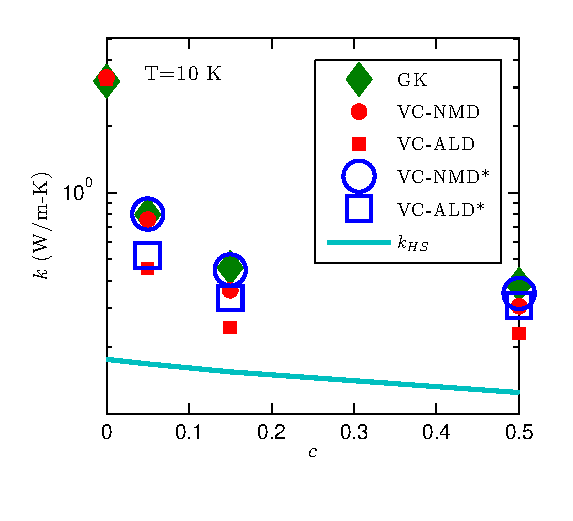
\includegraphics[scale=1.0]
{/home/jason/disorder/paper/vc/lj_cond_compare_2.eps}
\vspace*{-5mm}
\end{center}
\caption{\label{F:cond_lj} Thermal conductivity predictions for 
LJ argon and alloys at $T$=10 K using the VC-NMD, VC-ALD, and GK methods. 
The high-scatter thermal conductivity prediction $k_{HS}$ 
[Eq. \eqref{EQ:M:k_AF,HS}]  
and the high-scatter adjusted VC-NMD$^*$ and VC-ALD$^*$ are also plotted. 
}
\end{figure}
%--------------------------------------------------------------------------

%--------------------------------------------------------------------------
\begin{center}
%\begingroup
%\squeezetable
\begin{table}
\caption{\label{T:cond_table}Thermal conductivity predictions using the 
VC-NMD, VC-ALD, and GK methods. For LJ argon alloys, the bulk extrapolation 
is used for all three methods.  For SW silicon alloys, only VC-ALD and GK 
can be used to extrapolate a bulk thermal conductivity 
(see Section \ref{S:Thermal Conductivity}). For VC-NMD and GK, the 
uncertainties 
are estimated by omitting independent simulations from 
the ensemble averaging (see Section \ref{S:Calculation}). For VC-ALD, 
the uncertainties are estimated by omitting extrapolation points used for 
Eq. \eqref{EQ:k0}.}
\begin{ruledtabular}
\begin{tabular}{llllll}
$c$  ~~~~\vline GK ~~~~~~~~~~~ \vline VC-NMD~~~~\, \vline VC-ALD~~~~~\, \vline VC-NMD$^*$~~~ \vline VC-ALD$^*$ ~~\: \vline  \\
\hline
LJ  \\
\hline
0.00 \vline 3.3 $\pm$ 0.1 ~~~\, \vline 3.3 $\pm$ 0.1 ~~ \,\, \vline 3.4 $\pm$ 0.1 ~~~\,\,\, \vline ~~~~~~~~~~~~~~\;~\,\, \vline~~~~~~~~~~~~~\:\:\,\, ~ \vline \\
0.05 \vline 0.80 $\pm$ 0.07 \, \vline 0.76 $\pm$ 0.07 ~ \vline 0.45 $\pm$ 0.02 ~\, \vline 0.80 $\pm$ 0.1 \,  ~ \vline 0.52 $\pm$ 0.05  ~ \vline  \\
0.15 \vline 0.46 $\pm$ 0.07 \, \vline 0.36 $\pm$ 0.04 ~ \vline 0.24 $\pm$ 0.01 ~\, \vline 0.45 $\pm$ 0.05  ~ \vline 0.33 $\pm$ 0.07  ~ \vline  \\
0.50 \vline 0.38 $\pm$ 0.07 \, \vline 0.31 $\pm$ 0.04 ~ \vline 0.23 $\pm$ 0.01 ~\, \vline 0.35 $\pm$ 0.05  ~ \vline 0.31 $\pm$ 0.07  ~ \vline  \\
\hline
SW \\
\hline
0.00 \vline 520 $\pm$ 30 ~~~\, \vline ~~~~~~~~~~~~~~~~\; \vline 480 $\pm$ 20 ~~~~~ \vline ~~~~~~~~~~~~~~~~\; \vline~~~~~~~~~~~~~~~\:\:\: \vline  \\
0.05 \vline 20 $\pm$  2 ~~~~~~\, \vline ~~~~~~~~~~~~~~~~\; \vline 24 $\pm$ 2 ~~~~~~~~ \vline ~~~~~~~~~~~~~~~~\; \vline 24 $\pm$ 2 ~~~~~~\:\, \vline  \\
0.15 \vline 9.9 $\pm$ 0.9 ~~\;\, \vline ~~~~~~~~~~~~~~~~\; \vline 12 $\pm$ 1 ~~~~~~~~ \vline ~~~~~~~~~~~~~~~~\; \vline 12 $\pm$ 1 ~~~~~~\:\, \vline  \\
0.50 \vline 9.3 $\pm$ 0.9 ~~\;\, \vline ~~~~~~~~~~~~~~~~\; \vline 11 $\pm$ 1 ~~~~~~~~ \vline ~~~~~~~~~~~~~~~~\; \vline 11 $\pm$ 1 ~~~~~~\:\, \vline  \\
\end{tabular}
\end{ruledtabular}
\end{table}
%\endgroup
\end{center}
%--------------------------------------------------------------------------

% %--------------------------------------------------------------------------
% \begin{figure}
% \begin{center}
% \includegraphics[scale=1.0]
% {/home/jason/disorder/pbte/m_pbte_cond_compare.eps}
% \vspace*{-5mm}
% \end{center}
% \caption{\label{F:conductivity_lj} }
% \end{figure}
% %--------------------------------------------------------------------------

\clearpage

%--------------------------------------------------------------------------
\section{\label{S:SW}SW silicon}
%--------------------------------------------------------------------------

The failure of VC-ALD to predict the thermal conductivities of the LJ 
alloys is due to an underprediction of the high-frequency mode lifetimes, 
which make an important contribution to the thermal conductivity 
[see Sections \ref{S:Diffusivities} and \ref{S:Thermal Conductivity}, 
Figs. \ref{F:Dph_lj}(a) and \ref{F:Dph_lj}(c)]. To provide a contrast, 
we now predict the mode properties and thermal conductivity for bulk 
and alloyed SW silicon, where it is known that low-frequency modes 
dominate the thermal conductivity.
\cite{sellan_size_2010,sellan_cross-plane_2010} 
The lifetimes for the perfect crystal and an alloy with a concentration of 
0.5 predicted by VC-NMD and VC-ALD are plotted in Fig. \ref{F:Dph_si}(a). 
The VC-NMD predicted lifetimes are generally larger than 
the IR limit for SW silicon alloys, similar 
to the VC-NMD predictions for the LJ argon alloys 
(Fig. \ref{F:VC Gamma life}). Unlike the 
LJ argon alloys, the  
VC-NMD and VC-ALD predicted lifetimes agree over most 
of the frequency spectrum, except at the highest frequencies, where 
VC-ALD underpredicts VC-NMD and falls below the IR limit. 
The high-frequency plateau of the VC-NMD predicted lifetimes 
for LJ argon (Fig. \ref{F:VC Gamma life}) is not seen for SW silicon. 
As seen in Figs.~\ref{F:Dph_lj}(b) 
and \ref{F:Dph_si}(b), VC-NMD and VC-ALD both predict a significant 
number of modes with  
$D_{ph}\kv$ less than $D_{HS}$ for both the LJ argon and 
SW silicon alloys. 

The thermal conductivity spectrum for bulk SW silicon and an alloy 
with a concentration of 0.5 is plotted in Fig. \ref{F:Dph_si}(c). 
For bulk and the alloy, the thermal conductivity is dominated by 
low-frequency modes, so that large system-sizes are needed to satisfy 
the extrapolation requirements and only GK and VC-ALD can be used to 
predict a bulk value from Eq. \eqref{EQ:k0} ($N_0 \le 42$, similar 
to the converged system-sizes in Ref. \citenum{he_lattice_2012}). 
This system-size requirement highlights the efficiency of the 
VC-ALD method compared to VC-NMD, which is necessary when 
computationally-expensive DFT calculations are used.
\cite{esfarjani_method_2008,garg_role_2011,tian_phonon_2012,
lindsay_thermal_2012,esfarjani_heat_2011,chaput_phonon-phonon_2011}
The bulk thermal conductivity 
predictions for VC-ALD and GK are shown in Table \ref{T:cond_table} and 
plotted in Fig. \ref{F:cond_si}. The alloy thermal conductivities predicted 
by VC-ALD are $20\%$ larger than those from GK, in contrast to VC-ALD 
underpredicting for LJ argon alloys. This overprediction 
by VC-ALD compared to GK is close to the overprediction ($15\%$) of VC-ALD 
using DFT calculations of SiGe alloys compared to experiment 
without including disorder explicitly.\cite{garg_role_2011} 

The predicted thermal conductivities for the SW silicon alloys at 
all concentrations are over an order of magnitude larger than
the HS prediction, $k_{HS}$. Because the thermal transport in SW silicon 
is dominated by low-frequency modes, the HS adjustment  
VC-ALD$^*$ is within one percent compared 
to the unadjusted VC-ALD. 
While higher-order interactions in the Tamura theory 
may be responsible for the 
discrepancy of the lifetimes predicted by VC-NMD and VC-ALD in SW silicon 
at the highest frequencies [Fig. \ref{F:Dph_si}(a)],  
this effect is not important to the overall
thermal transport. VC-ALD predicts accurate alloy thermal 
conductivities for SW silicon because it is a low-frequency 
dominated material, which is the frequency range where the standard 
application of the Tamura theory is valid.\cite{tamura_isotope_1983} 

%--------------------------------------------------------------------------
\begin{figure}
\begin{center}
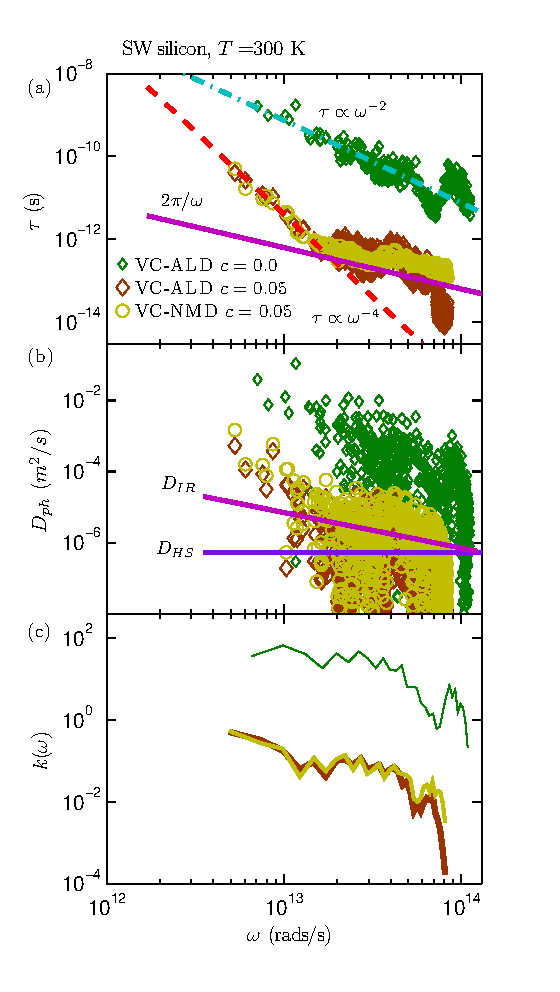
\includegraphics[scale=1.0]
{/home/jason/disorder/paper/vc/af_nmd_ald_tau_diff_kw_c5-2.eps}
\vspace*{-5mm}
\end{center}
\caption{\label{F:Dph_si} (a) Predicted lifetimes using VC-NMD and VC-ALD 
for SW silicon ($T=300$ K, $N_0=8$ and $c=0.05$).  
(b) Mode diffusivities compared  
to the HS limit, $D_{HS}$ [Eq. \eqref{EQ:M:D_HS}], 
and the IR limit, $D_{IR}$ [Eq. \eqref{EQ:M:D_IR}]. 
VC-NMD and VC-ALD predict a large number of high-frequency modes 
with $D_{ph} < D_{HS}$, as 
seen in the LJ argon alloys [Fig. \ref{F:Dph_lj}(b)]. 
(c) Thermal conductivity frequency spectrum, 
which peaks at low frequency, in contrast to LJ argon 
[Fig. \ref{F:Dph_lj}(c)].
}
\end{figure}
%--------------------------------------------------------------------------

%--------------------------------------------------------------------------
\begin{figure}
\begin{center}
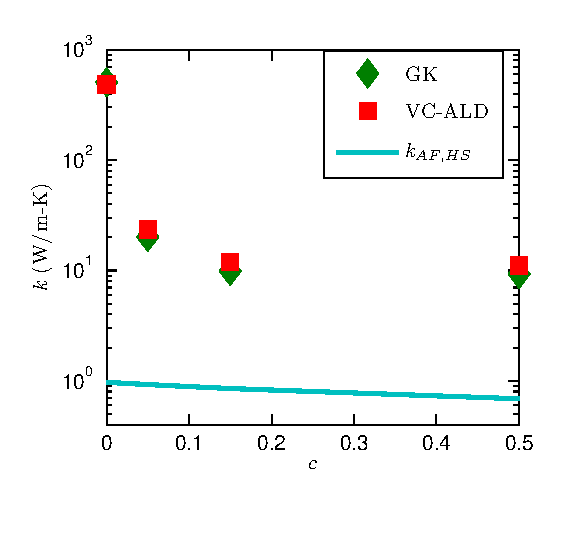
\includegraphics[scale=1.0]
{/home/jason/disorder/paper/vc/m_si_cond_compare.eps}
\vspace*{-5mm}
\end{center}
\caption{\label{F:cond_si}Thermal conductivity predictions for 
SW silicon and alloys at a temperature of 300 K using the VC-ALD and 
GK methods. 
The high-scatter thermal conductivity prediction $k_{HS}$ 
is also plotted. 
The adjusted VC-ALD$*$ is not shown since it differs by only one 
percent compared to VC-ALD.}
\end{figure}
%--------------------------------------------------------------------------

\clearpage

% %--------------------------------------------------------------------------
% \section{\label{S:Discussion}Thermal Properties Discussion}
% %--------------------------------------------------------------------------

% The VC approximation underpredicts 
% the mode thermal 
% diffusivity due to disorder because the group velocities $v_g\kv$ can 
% approach zero (Section ), though this is a small effect compared to 
% the underprediction of the lifetimes by VC-ALD. 

% As observed by Kittel, if the sound
% velocity is used instead of U; and the interatomic spacing
% is used instead of the mean free path l;, then tc( T) is qual-
% itatively and semiquantitatively
% fit at temperatures above
% the plateau region.
% In fact, Slack showed that the same model 
% is useful for crystalline insulators with strong scattering.(waiting for 
% ILL).\cite{henry_ehrenreich_thermal_1979}

% The theory by Tamura is able to treat disorder scattering in an arbitrary 
% crystal with dispersion. The theory, however, fails to predict the 
% lifetimes of high-frequency modes, which are critical to the total 
% thermal conductivity in LJ argon (see Fig. and ). To match the predicted 
% phonon lifetime at high fequency for $c=0.05$ 
% ($\tau\kv \propto const.$, Fig. ), 
% the Tamura theory (to order 2, $g_2(b)$) requires a DOS which scales as 
% $D(\omega\kv) \propto const.$. Clearly from Fig. , this is not the case 
% with either the VC or Gamma modes. To match the predicted 
% phonon lifetime at high fequency for $c=0.5$ 
% ($\tau\kv \propto 1/\omega\kv$, Fig. , also true for all $c$ in SW silicon), 
% The higher-order terms in the Tamura theory are demonstrated to be large 
% in Fig., but it is unclear if and how they are responsible for the 
% underpredictions of the VC-ALD method for LJ argon. 

% While Broido found that omission of optical scattering overpredicts 
% the thermal 
% conductivity of bulk Si by a factor of 2-3, 
% optical modes contribute less than $5\%$ 
% to thermal conductivity itself. Similarly, the diffusivity adjusted 
% thermal 
% cobductivities of SW Si are increased by less then about $1\%$, 
% demonstrating the 
% the high frequency and optical modes are also unimportant to thermal 
% transport 
% in Si alloys. 

% For the perfect system, phonon modes with nearly zero group velocity 
% (optical modes and acoustic modes at the BZ boundaries) have essentially 
% zero thermal diffusivity and contribute nearly 
% nothing to the thermal transport, while the modes themselves 
% are important to the 
% scattering of other phonons.(cite) In the disordered lattices under the 
% AF theory, modes important to thermal transport have a finite thermal 
% diffusivity, as opposed to  the minimum $D_{th} \approx 0 $ for phonons 
% in a perfect lattice. This finite thermal diffusivity limit is the cause 
% for the large (LJ argon Fig. ) and small (SW silicon Fig. ) 
% descrepcny between the thermal conductivity prdictions of VC-ALD and 
% VC-NMD versus 

% High thermal conductivity materials tend to have a conductivity spectrum 
% which is peaked in the low frequency range.(cite) 
% It is in this range where the mode 
% lifetimes follow closely the scalings with frequency which can be 
% predicted by the perturbative models for intrinsic and disorder 
% scattering as 
% (Section Eq. ).

% In contrast, 
% in LJ argon the high frequency phonon mode properties are critical 
% to the thermal transport.(cite)  
% While the low frequency phonon properties predicted by VC-NMD and 
% VC-ALD agree, it is the failure of the perturbative models at 
% high frequency which causes VC-ALD to underpredict. The failure 
% to account for harmonic disordered scattering due to the AF theory 
% is responsible for causing both VC-NMD and VC-ALD to underpredict 
% versus GK, which affects the high frequency modes significantly. 
% LJ argon, with lower 
% frequencies, lifetimes, and group velocities compared to 
% ``stiff'' SW silicon, 
% is considered a ``soft'' system. 

% For SW silicon, the low frequency modes dominate thermal transport 
% even in the heavily disordered alloy.(cite new Hopkins) 
% It is thus unsurprising that predictions for 
% SW silicon using VC-ALD agree well with VC-NMD and GK. This is also a 
% plausible explanation for the success of predictions using 
% VC-ALD and ab initio calculations compared to experiment for 
% ``stiff'' systems (i.e. Si-Ge).(cite)

%--------------------------------------------------------------------------
\section{\label{S:Summary}Summary}
%--------------------------------------------------------------------------

In this study, we investigated the use of the VC 
approximation for predicting the vibrational mode properties and 
thermal conductivity of LJ argon and SW silicon alloys 
by a detailed comparison of the VC-NMD, VC-ALD, and GK methods. 
By using computationally-inexpensive  
empirical potentials we self-consistently studied the effects of 
disorder both explicitly (Sections \ref{S:VC Gamma DOS}, 
\ref{S:Dispersion},  
\ref{S:From VC Gamma}, \ref{S:Diffusivities}, and \ref{S:SW}) 
and as a perturbation (Sections \ref{S:From VC-ALD} and \ref{S:SW}). 
By spanning a range of disorder, the limits of the 
perturbative models were examined.
A breakdown of the VC-ALD method was identified for LJ argon alloys 
by a comparison with the VC-NMD method in 
Section \ref{S:From VC-ALD}   
and a correction was suggested in Section \ref{S:Thermal Conductivity}. 
The mode properties and thermal 
conductivity of the SW silicon alloys were predicted and in 
Section \ref{S:SW} and provided a contrast to the 
LJ argon alloys, which have a different thermal conductivity 
spectrum. 

The results for the SW silicon and LJ argon alloys suggest that 
modeling of thermal transport in ordered and 
disordered lattices can be separated into two broad groups: 
low-frequency dominated and full-spectrum materials.  
Materials dominated by low-frequency modes tend to have high 
thermal conductivities that are significantly larger than the 
HS limit [Eq. \eqref{EQ:M:k_AF,HS}], 
which is due to the large group velocities and long lifetimes 
of low-frequency modes.\cite{abeles_thermal_1962,
abeles_lattice_1963,kamitakahara_vibrations_1974,
cahill_thermal_2004,cahill_thermal_2005,garg_role_2011,
lindsay_thermal_2012,cheaito_experimental_2012} 
These low-frequency modes  
closely follow the scalings predicted by the perturbative VC-ALD 
models, which are valid at low-frequencies. 

LJ argon is a material whose thermal transport has significant 
contribution from high-frequency modes, even for the bulk 
[see Fig. \ref{F:Dph_lj} (c)]. 
This high-frequency range is where we predict that the 
perturbative Tamura theory   
will have non-negligible contributions from higher-order 
interactions (see Section \ref{S:From VC-ALD}). 
While the higher-order interactions in the 
Tamura theory are also predicted to be 
non-negligible for SW silicon, this does not affect the thermal 
conductivity predictions significantly because high-frequency modes  
are not important to thermal transport. The negligible contributions 
of high-frequency modes is demonstrated by experimental measurements 
of the thermal conductivity of SiGe alloys, which exceed the HS limit 
by more than an order of magnitude at room temperature for all 
compositions.
\cite{cahill_lattice_1988,cahill_thermal_2004,
cahill_thermal_2005,cheaito_experimental_2012} Experimentally-accurate 
theoretical predictions\cite{garg_role_2011} 
also demonstrate that high-frequency modes 
are unimportant to thermal transport, 
although they do serve as important scattering channels.
\cite{ward_intrinsic_2010} 

The VC-ALD method provides a computationally inexpensive framework, 
which is 
essential when using \emph{ab initio} 
methods for predicting thermal conductivity.
\cite{ward_intrinsic_2010,lindsay_thermal_2012,
garg_role_2011,
shiga_microscopic_2012,tian_phonon_2012,
shiomi_thermal_2011,esfarjani_heat_2011,
li_thermal_2012,luckyanova_coherent_2012} Based on our results, 
we believe that the Tamura theory breaks down for mode  
diffusivities predicted to be below the HS limit, $D_{HS}$ 
[Eq. \eqref{EQ:M:D_HS}]. 
This breakdown may be true for the high-frequency modes of any 
disordered lattice\cite{sheng_heat_1991} 
and the high-scatter limit $D_{HS}$ should be 
considered whenever the perturbative VC-ALD method is used.
Although the HS limit of 
diffusivity is usually interpreted as a minimum mean free path,
\cite{kittel_interpretation_1949,graebner_phonon_1986,
cahill_lattice_1988,sheng_heat_1991} 
we find that this concept is not necessary for interpreting the results 
of this work. In a disordered lattice, the fundamental quantities are 
the mode lifetime and diffusivity\cite{sheng_heat_1991,allen_thermal_1993,
allen_diffusons_1999,taraskin_determination_1999} and the 
VC predicted group velocity is an approximation.

\begin{acknowledgements}
This work was supported by AFOSR award FA95501010098 and by a grant 
of computer time from the DOD 
High Performance Computing Modernization Program at the US Army Engineer 
Research and Development Center. 
We thank Davide Donadio, Jivtesh Garg, Asad Hasan, Craig Maloney, 
and Zhiting Tian for helpful discussions.
\end{acknowledgements}

%--------------------------------------------------------------------------
\appendix
%--------------------------------------------------------------------------

% %--------------------------------------------------------------------------
% \section{\label{A:Computational Cost}
% Computational Cost}
% %--------------------------------------------------------------------------
% 
% The key to incorporating the effects of disorder explicitly are the use 
% of a large disordered supercells (Section \ref{S:Calculation}). 
% However, the methods used 
% in this work scale differently with the size of the supercell considered. 
% The calculations in this work are trivially parallelizable\cite{} 
% except the 
% MD simulations\cite{plimpton_fast_1995} and the eigenvalue solution of the 
% Dynamical matrix.\cite{gale_general_2003} Efficient MD 
% codes scale linearly with the number of atoms in the system $N_a$, making 
% the GK method an efficient method for predicting thermal conductivity. 
% However, the computational cost of using large supercells for MD simulation, 
% particularly because of the large number of time steps required 
% (on the order of $10^5 - 10^7$ depending on the 
% system, time step used, etc (cite)), prohibit its use with typical 
% \emph{ab initio} methods such as 
% plane-wave Density Functional Theory.(cite) 
% 
% Both VC-NMD and VC-ALD require the eigenvalue solution 
% of a Dynamical matrix of size $(3n,3n)$ for each irreducible wavevector 
% of the system size considered, 
% which is negligible compared to the other 
% caculations required for both of these methods.(cite) 
% The Gamma-NMD (Section \ref{S:VC Gamma life}) and 
% AF theory (Section \ref{S:Diffusivities}) 
% require the eigenvalue solution of a large Dynamical matrix $(3N_a,3N_a)$, 
% the solution of which scales as $(3N_a)^3$. 
% The AF theory is limited 
% to small supercells using ab initio calculations, making it difficult 
% to asses finite-size effects.(cite)  
% 
% Using the VC-ALD method, the symmetries of the system can be 
% used to drastically reduce the required computations, permitting its 
% use with ab initio methods.
% \cite{esfarjani_method_2008,turney_predicting_2009,
% esfarjani_heat_2011,chaput_phonon-phonon_2011} 
% For VC-ALD, the calculation of the intrinsic phonon 
% lifetimes $\tau_{p-p}\kv$ scales as $n^4$,\cite{turney_predicting_2009}  
% making calculations for large unit cells challenging.(cite) 
% Compared to 
% the calculation of the intrinsic phonon lifetimes, calculation 
% of the defect lifetimes $\tau_d\kv$ (Eq. ) is negligible.

% Consider the following computational times for the methods used in 
% this work for LJ argon and $N_0 = 12$. All calculations were performed 
% on the same computing cluster and include the effect of using 
% multiple processors (for example the VC-ALD calculations were run using 
% 12 cpu for 4.1 hours):
% 
% AF = eigenvalue solution + thermal diffusivity calculation = 4.2 hours
% 
% VC-ALD time = 49.2 hours?
% 
% VC-NMD time = 102 hours for MD + 780 hours for NMD + negligible time 
% to generate phonon frequencies and eigenvectors
% 
% LJ VC-Gamma = MD simulation + NMD + eigenvalue solution =  
% 102 hours + 780 hours + 3.8 hours = 
% 
% Parallel eigenvalue solvers exist for most ab initio packages, required 
% to solve for the eigenvalues of the Hamiltonian matrix.(cite) Incorporating 
% parallel eigenvalue solvers into existing 
% Sparse eigenvalue solutions may be implemented for systems which are 
% large enough and have short-range interactions.(cite)

% \begin{center}
% \begin{table}
% \caption{\label{T:cond_table}Thermal conductivity values in W/m-K predicted using the $\Phi$, 
% $\Phi'$, and Green-Kubo methods.  The predictions for $\Phi$ and Green-Kubo for the LJ system 
% are in good agreement with those from other atomistic simulation methods\cite{turney2009a} while 
% those from $\Phi'$ differ and show no consistent behavior. The uncertainties in the predicted thermal 
% conductivities for $\Phi$ and $\Phi'$ come predominantly from the finite simulation-size scaling 
% procedure (see Ref. \cite{turney2009a,He2011a}), where the phonon properties and thermal conductivity 
% are predicted for increasing system sizes ($N_1=N_2=N_3$) to extrapolate a bulk thermal conductivity. 
% For SW silicon and the CNT, the extrapolation procedure is not performed. }
% \begin{ruledtabular}
% \begin{tabular}{llllll}
%      &                             &         &      &   \\
% $T$ (K)&Green-Kubo \ &$\Phi$ &$\Phi'$\\
% \hline
% LJ (bulk)\\
% 5&8.0 $\pm$ 0.30 &7.9 $\pm$ 0.42 &5.8 $\pm$ 0.31 \\
% 20&1.3 $\pm$ 0.15 &1.2 $\pm$ 0.07 &1.0 $\pm$ 0.10 \\
% 40&0.45 $\pm$ 0.07 &0.47 $\pm$ 0.03 &0.49 $\pm$ 0.05 \\
% \hline
% SW ($N_1=N_2=N_3=6$) \\
% 300& &322 $\pm$ 16 &396 $\pm$ 38 \\
% \hline
% CNT ($N_1=N_2=1, N_3=50$) \\
% 300& &428 $\pm$ 21 &398 $\pm$ 40 \\
% \end{tabular}
% \end{ruledtabular}
% \end{table}
% \end{center}

%MD: Loop time of 2021.86 on 12 procs for 1000000 steps with 6912 atoms
%matlab NMD: /home/jason/lammps/LJ/alloy/10K/0.5/12x/NMD/1
%35261.719809 for one NMD_1_1

%--------------------------------------------------------------------------
\section{\label{A:NMD XCORR}
NMD using Non-Exact Normal Modes}
%--------------------------------------------------------------------------

For a normal mode of the lattice supercell 
used for the MD simulations (i.e., a Gamma mode), 
the total energy autocorrelation is an exponential function  
with a decay time $\tau\kv$ and the kinetic energy autocorrelation is a 
exponentially-damped sinusoidal oscillation with frequency 
$2\omega\kv$.\cite{mcgaughey_predicting_2013} 
When projecting MD simulations  
of the explicitly disordered lattice supercells 
onto the VC normal modes, 
the energy autocorrelation functions 
do not always follow the simple functional forms, 
as shown in Fig. \ref{F:NMD XCORR} for two modes in the LJ alloy at a 
concentration of 0.5.  
By calculating the mode kinetic energy in the  
frequency-domain, $\Phi$,\cite{larkin_comparison_2012} artifacts such as 
multiple peaks are observed (see main plot).   

These artifacts are not surprising given two considerations: 
(i) the MD simulations 
contain explicit disorder that influences the atomic trajectories, 
and (ii) the VC-normal modes are not the exact normal modes of the 
explicitly-disordered lattice supercells. 
An effective lifetime can be predicted 
using Eq. \eqref{EQ:tau_nmd} 
because the VC total mode energy autocorrelations 
still decay to zero in a finite time. This results is to be expected 
given that the atomic trajectories contain 
information about the lattice energy, which from general statistical 
physics principles will have exponential relaxation behavior in an 
equilibrium ensemble.
\cite{landau_statistical_1980,srivastava_physics_1990,
rajabpour_thermal_2010}

%--------------------------------------------------------------------------
\begin{figure}
\begin{center}
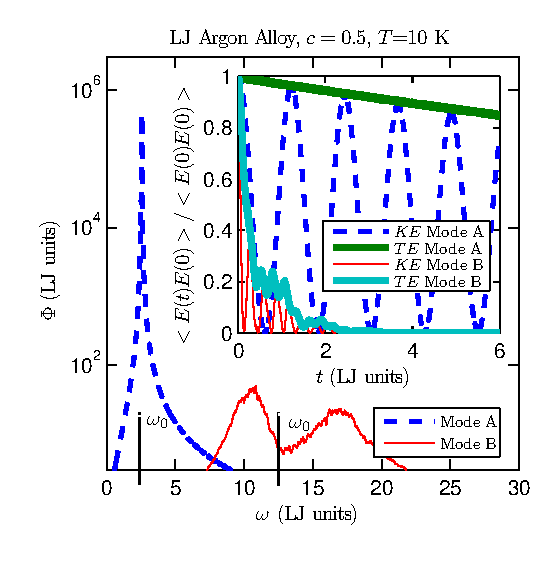
\includegraphics[scale=1.0]
{/home/jason/disorder/paper/vc/m_lj_nmd_xcorr_compare_2.eps}
\vspace*{-5mm}
\end{center}
\caption{\label{F:NMD XCORR} The normal mode kinetic energy, $\Phi$,  
of two modes (A and B) at wavevector [0.25 0 0] calculated 
using VC-NMD for a mass disordered LJ FCC supercell 
($N_0=8$ and $c=0.5$) is shown in the main figure. 
The VC dispersion-predicted peaks are labeled 
by $\omega_0$. The inset shows the same mode's energy 
[kinetic ($KE$) and total ($TE$)] autocorrelation functions.  
Note the additional oscillation effects in the KE and TE autocorrelation 
functions for Mode B which are due to the two peaks in $\Phi$. 
A mode lifetime can 
be extracted unambiguously using the integral of the TE autocorrelation 
function [Eq. \eqref{EQ:tau_nmd} in Section \ref{S:From VC Gamma}].}
\end{figure}
%--------------------------------------------------------------------------


% %--------------------------------------------------------------------------
% \section{\label{A:SF}Calculation of the Gamma Mode Structure Factors}
% %--------------------------------------------------------------------------
% 
% To calculate 
% $S^{L,T}\kw$ for a finite-size system, the 
% delta function in Eq. \eqref{EQ:M:SLT} is broadened using a Lorentzian 
% function with a full-width at half maximum 
% $\Gamma_{FMHW} = \delta_{\omega,avg}$, 
% where 
% $\delta_{\omega,avg}$ is the average frequency spacing. 
% Allen et al\cite{allen_diffusons_1999} 
% demonstrated using a model of 
% a-Si that the structure factor 
% for large wavevector broadens so that the 
% linewidth $\Gamma_{SF} > \omega$.
% \cite{taraskin_determination_1999}
% For the systems sizes studied, $\Gamma_{SF}$ 
% scale with the broadening factor 
% $\Gamma_{FMHW}$ for all peaks 
% except those at high frequencies. 
% 
% For the range of broadening factors 
% considered ($\Gamma_{FMHW} = \delta_{\omega,avg}$ to $50\delta_{\omega,avg}$) 
% the linedwidths extracted for all $c$ 
% generally satisfy $\Gamma_{SF} > \omega$. 
% For all broadening factors, the linewidths 
% (inverse lifetimes, $\tau_{SF} = 1/2\Gamma_{SF}$) 
% at high frequency are in better 
% agreement with the lifetimes predicted 
% by VC-NMD rather than VC-ALD,
% where generally $\tau > 2\pi/\omega$ 
% (IR limit, Fig. \ref{F:VC Gamma life}).
% \cite{taraskin_determination_1999} This gives more  
% justification for the use of the VC predicted group velocities for 
% both VC-NMD and VC-ALD, even for large wavevector and $c$. 
% 
% In general, the polarization of the eigenvectors $e\kvba$ will not 
% be purely transverse or longitudinal along the reciprocal directions. 
% Even for the simple LJ argon system, this can make it difficult to 
% uniquely identify then different polarizations with the various 
% peaks in the structure factors. For SW silicon, similar good agreement 
% can be seen along the high symmetry directions for the acoustic branches, 
% while the optical modes 
% and more complicated polarizations are too difficult to identify in 
% an automated way. 
% In general, the acoustic branches can be identified, provided they are 
% well separated in frequency from any optical branches.
% \cite{feldman_numerical_1999,thomas_predicting_2010} 

% %--------------------------------------------------------------------------
% \section{\label{A:Finite Simulation}
% Finite Simulation-Size Scaling for Thermal 
% Conductivity}
% %--------------------------------------------------------------------------
% To predict a bulk thermal conductivity, extrapolation is used by the 
% following finite size scaling $ 1 / k \propto 1/N_0$. For VC-NMD and 
% VC-ALD, the validity of the finite-size scaling 
% requires the low frequency modes in the finite system to be dominated by 
% intrinsic scattering ($\tau\kv \propto \omega\kv^{-2}$) and  
% follow the Debye approximation 
% with respect to $v_{g,\mathbf{n}}$ and DOS $D(\omega\kv)$.
% \cite{shiomi_thermal_2011,esfarjani_heat_2011} For LJ 
% argon, this requirement is satisfied for modest system sizes 
% (for $N_0 = 6$ to $12$) so that both VC-NMD and VC-ALD predictions 
% can be extrapolated to a bulk value. 
% For SW silicon, the thermal conductivity is dominated by low-frequency 
% modes (Fig. \ref{F:Dph_si}). Becasue of this, large system sizes 
% (up to $N_0 = 42$) are needed to satisfy the 
% extrapolation requirements and only VC-ALD can be used.(cite) This 
% demonstrates the computational efficient of the VC-ALD method which is 
% necessary when computationally expensive 
% ab initio methods are used (Section ).
% \cite{garg_role_2011,tian_phonon_2012,
% lindsay_thermal_2012,esfarjani_heat_2011}
% 
% System sizes of up to $N_0=38$ are required to predict converged 
% thermal conductivity of SW silicon alloys. 
% For Si modeled using the Tersoff potential, 
% system sizes of up to 64000 atoms are required to observe 
% converged values of thermal conductivity using the GK method.
% \cite{he_lattice_2012} We find that similar system sizes are 
% also required for 
% 
% For the GK method, smaller system sizes $N_0 \le 12$ are used for the 
% finite size extrapolation for LJ argon and SW silicon . 
% The validity of this result can be explained in terms of a 
% combination of effects which are specific to the MD simulations.
% \cite{esfarjani_heat_2011} In fact, for $c=0$ the GK results are 
% independent of system size for $N_0 = 4$ to $N_0 = 12$ for LJ argon.

\clearpage
\bibliographystyle{apsrev}
%\bibliography{/home/jason/sed/jop/asme_prb_paper/prb/references}
\bibliography{/home/jason/disorder/paper/vc/ntpl-032013}
\end{document}
